\documentclass[output=paper
,modfonts
,nonflat]{langsci/langscibook} 
%\bibliography{localbibliography}
%% add all extra packages you need to load to this file 
\usepackage{graphicx}
\usepackage{tabularx}
\usepackage{amsmath} 
\usepackage{multicol}
\usepackage{lipsum}
%%%%%%%%%%%%%%%%%%%%%%%%%%%%%%%%%%%%%%%%%%%%%%%%%%%%
%%%                                              %%%
%%%           Examples                           %%%
%%%                                              %%%
%%%%%%%%%%%%%%%%%%%%%%%%%%%%%%%%%%%%%%%%%%%%%%%%%%%%
% remove the percentage signs in the following lines
% if your book makes use of linguistic examples
\usepackage{langsci/styles/langsci-gb4e} 
\usepackage{langsci/styles/langsci-optional} 
\usepackage{langsci/styles/langsci-lgr}
\usepackage{langsci/styles/langsci-bidi}
\usepackage{morewrites} 
%% if you want the source line of examples to be in italics, uncomment the following line
% \def\exfont{\it}

%\usepackage{enumitem} %Conflict with enumerate
\usepackage{lipsum}
\usepackage{multirow}
\usepackage{graphicx}
\usepackage{epstopdf}
\usepackage{wrapfig}
\usepackage{caption}
\usepackage{subcaption}
\usepackage{url}
\usepackage{relsize}
\usepackage{paralist}
\usepackage{tabularx} 
%\newfontfamily\Parsifont[Script=Arabic]{langsci/fonts/ScheherazadeRegOT_Jazm.ttf} 
\usepackage{latexsym}
\usepackage{tikz-dependency}
\usepackage{textgreek}
\usepackage{color}
\usepackage{newfloat}
\usepackage{hhline}
\usepackage{xspace}
\usepackage{booktabs}
\usepackage{verbatim} 
\usepackage{algorithm}
\usepackage[noend]{algpseudocode}
\usepackage{sidecap}
\usepackage{kantlipsum}
\usepackage{verbatimbox} 
\usepackage[usestackEOL]{stackengine}
\usepackage{tikz}
\usetikzlibrary{shapes.arrows}
\usepackage{todonotes}
\usepackage{csquotes}
\usepackage{amsmath}
%\usepackage[british]{babel}
\usepackage{mathtools}  % better amsmath
\usepackage{dcolumn}
\newcolumntype{d}[0]{D{.}{.}{2}}
\usepackage{cjhebrew} % Hebrew
\usepackage[normalem]{ulem}
\usepackage{qtree}
\usepackage{rotating}
\usepackage[section]{placeins} 
\usepackage{soulutf8}  % \ul command for underlining
% \usepackage{langsci/styles/langsci-bidi}

\usepackage{booktabs} %Salehi et al.
\usepackage{makecell} %Bhatia


%%% hyphenation points for line breaks
%% Normally, automatic hyphenation in LaTeX is very good
%% If a word is mis-hyphenated, add it to this file
%%
%% add information to TeX file before \begin{document} with:
%% %% hyphenation points for line breaks
%% Normally, automatic hyphenation in LaTeX is very good
%% If a word is mis-hyphenated, add it to this file
%%
%% add information to TeX file before \begin{document} with:
%% %% hyphenation points for line breaks
%% Normally, automatic hyphenation in LaTeX is very good
%% If a word is mis-hyphenated, add it to this file
%%
%% add information to TeX file before \begin{document} with:
%% \include{localhyphenation}
\hyphenation{
affri-ca-te
affri-ca-tes
an-no-tated
com-ple-ments
com-po-si-tio-na-li-ty
non-com-po-si-tio-na-li-ty
Gon-zá-lez
out-side
Ri-chárd
se-man-tics
STREU-SLE
}
\hyphenation{
affri-ca-te
affri-ca-tes
an-no-tated
com-ple-ments
com-po-si-tio-na-li-ty
non-com-po-si-tio-na-li-ty
Gon-zá-lez
out-side
Ri-chárd
se-man-tics
STREU-SLE
}
\hyphenation{
affri-ca-te
affri-ca-tes
an-no-tated
com-ple-ments
com-po-si-tio-na-li-ty
non-com-po-si-tio-na-li-ty
Gon-zá-lez
out-side
Ri-chárd
se-man-tics
STREU-SLE
}
%%add all your local new commands to this file

\newcommand{\smiley}{:)}

\renewbibmacro*{index:name}[5]{%
  \usebibmacro{index:entry}{#1}
    {\iffieldundef{usera}{}{\thefield{usera}\actualoperator}\mkbibindexname{#2}{#3}{#4}{#5}}}

% \newcommand{\noop}[1]{}

%add all your local new commands to this file

\newcommand{\ie}{i.e., }

% \newcommand{\noop}[1]{}

\newcommand{\blex}[1]{\textit{#1}\xspace}

\newcommand{\ngram}[1][]{$n$-gram{#1}\xspace}

\newcommand{\mwetype}[1]{\texttt{#1}\xspace}
\newcommand{\strongish}{\mwetype{strong}}
\newcommand{\weak}{\mwetype{weak}}
%\newcommand{\hard}{\mwetype{hard}}
\newcommand{\hard}{\textit{hard}}
%\newcommand{\mixed}{\mwetype{mixed}}
\newcommand{\mixed}{\textit{mixed}}

\newcommand{\gap}{$*$\xspace}
\newcommand{\zp}{\phantom{0}}

\newcommand{\figureref}[1]{Figure~\ref{#1}\xspace}
\newcommand{\tableref}[1]{Table~\ref{#1}\xspace}
\newcommand{\sectionref}[1]{Section~\ref{#1}\xspace}


\DeclareFloatingEnvironment[fileext=lod]{diagram}
\newcommand{\nothing}[1]{}

\DeclareOldFontCommand{\bf}{\normalfont\bfseries}{\mathbf}
\DeclareOldFontCommand{\it}{\normalfont\bfseries}{\mathbf}
\DeclareOldFontCommand{\sc}{\normalfont\bfseries}{\mathbf}


% \newcommand{\noop}[1]{}


\newcommand{\class}[1]{\texttt{#1}\xspace}
\newcommand{\localex}[1]{\textit{#1}\xspace}
\newcommand{\gl}[1]{``{#1}''\xspace}

\newcommand{\x}{\phantom{0}}

% Style guide provides these...

\newcommand{\localtabref}[2][]{Table#1~\ref{#2}\xspace}
\newcommand{\secref}[2][]{Section#1~\ref{#2}\xspace}
\newcommand{\localfigref}[2][]{Figure#1~\ref{#2}\xspace}

\newcommand{\eqnref}[2][]{Equation#1~\ref{#2}\xspace}

\newcommand{\REDDY}{ENC\xspace}
\newcommand{\BANNARD}{EVPC\xspace}

\newcommand{\MWE}{\ensuremath{\mathit{mwe}}}
\newcommand{\component}{\ensuremath{\mathit{component}}}

\newcommand{\spadeaff}{\ensuremath{\spadesuit}\xspace}
\newcommand{\clubaff}{\ensuremath{\clubsuit}\xspace}
\newcommand{\heartaff}{\ensuremath{\heartsuit}\xspace}
\newcommand{\diamondaff}{\ensuremath{\diamondsuit}\xspace}


\newcommand{\CS}[1]{\ensuremath{\mathit{CS}_{\mathit{#1}}}\xspace}

\newcommand{\CSsource}{\CS{L1}}
\newcommand{\CStarg}{\CS{L2N}}
\newcommand{\CSsourcetarg}{\CS{L1+L2N}}
\newcommand{\CSsvr}{\CS{SVR(L1+L2)}}
\newcommand{\CSstring}{\CS{string}}
\newcommand{\CSall}{\CS{all}}
\newcommand{\CSstringDS}{\CS{string+L1}}

%add all your local new commands to this file

\newcommand{\main}[1]{\textbf{#1}}

%\newcommand{\dataset}[1]{\textsc{#1}\xspace}

%\newcommand{\dataset}[1]{\textsc{#1}}

\newcommand{\feat}[1]{{\textsc{#1}}}
\newcommand{\swfeat}[2]{\feat{#1$_{#2}$}}
\newcommand{\bgfeat}[3]{\feat{#1$_{#2}$#1$_{#3}$}}
\newcommand{\tgfeat}[4]{\feat{#1$_{#2}$#1$_{#3}$#1$_{#4}$}}

\newcommand{\best}[1]{\textbf{#1}}
\newcommand{\hd}[1]{\textbf{#1}}


\newcommand{\dev}{\textsc{dev}}
\newcommand{\devAQ}{\dev$_{AQ}$}
\newcommand{\devDD}{\dev$_{DD}$}

\newcommand{\full}{\textsc{full}}
\newcommand{\fullAQ}{\full$_{AQ}$}
\newcommand{\fullDD}{\full$_{DD}$}

\newcommand{\expl}[1]{\emph{#1}}
% \mwegloss{original}{literal}{translat}
\newcommand{\mwegloss}[3]{\expl{#1} (lit.\ \expl{#2}) `#3'}


\renewbibmacro*{index:name}[5]{%
  \usebibmacro{index:entry}{#1}
    {\iffieldundef{usera}{}{\thefield{usera}\actualoperator}\mkbibindexname{#2}{#3}{#4}{#5}}}

% \newcommand{\noop}[1]{}

\newcommand{\compresslist}{
\setlength{\itemsep}{1pt}
\setlength{\parskip}{0pt}
\setlength{\parsep}{0pt}
\setlength{\leftmargin}{10cm}
}

\newcommand{\revcr}[1]{\textcolor{black}{#1}} % Revised by Carlos Ramisch
\newcommand{\revms}[1]{\textcolor{black}{#1}}  % Revised by Manon Scholivet
\newcommand{\revsc}[1]{\textcolor{black}{#1}}     % Revised by Silvio Cordeiro


\newcommand{\mcomment}[2]{\noindent{{\scriptsize\sffamily(\marginpar{\sffamily #1}#2)}}}
\newcommand{\ncomment}[2]{\noindent{{\sffamily\marginpar{\sffamily #1}#2}}}

%\newcommand{\car}[1]{\mcomment{\tiny{CAR}}{\textcolor{green}{#1}}} %Carlos' comments
%\definechangesauthor[name={Carlos Ramisch}, color={Green}]{cr}
\newcommand{\as}[1]{\mcomment{\tiny{AS}}{\textcolor{blue}{#1}}} %Agata's comments
\newcommand{\cara}[1]{\mcomment{\tiny{CR}}{\textcolor{red}{#1}}} %Carlos' comment
\newcommand{\mc}[1]{\mcomment{\tiny{MC}}{\textcolor{orange}{#1}}} %Marie's comments
\newcommand{\vv}[1]{\mcomment{\tiny{VV}}{\textcolor{gray}{#1}}} %Veronika's comments
\newcommand{\src}[1]{\mcomment{\tiny{SRC}}{\textcolor{magenta}{#1}}} %Silvio's comments
\newcommand{\fs}[1]{\mcomment{\tiny{FS}}{\textcolor{brown}{#1}}} %Federico's comments
\newcommand{\ad}[1]{\mcomment{\tiny{AD}}{\textcolor{brown}{#1}}} %Antoine's comments
\newcommand{\fc}[1]{\mcomment{\tiny{FC}}{\textcolor[rgb]{.7,0,.2}{#1}}} %Fabienne's comments
\newcommand{\iva}[1]{\mcomment{\tiny{IS}}{\textcolor{yellow}{#1}}} %Iva's comments
\newcommand{\bqz}[1]{\mcomment{\tiny{BQZ}}{\textcolor{gray}{#1}}} %Behrang's comments
\newcommand{\vg}[1]{\mcomment{\tiny{VG}}{\textcolor{magenta}{#1}}} %Voula's comments
\newcommand{\kuad}[1]{\mcomment{\tiny{KA}}{\textcolor{green}{#1}}} %Kübra's comments
\newcommand{\eb}[1]{\mcomment{\tiny{EB}}{\textcolor[rgb]{.3,.7,.2}{#1}}} %Eduard's comments
\newcommand{\guer}[1]{\mcomment{\tiny{GE}}{\textcolor{Mahogany}{#1}}} %Gulsen's comments
\newcommand{\jm}[1]{\mcomment{\tiny{JM}}{\textcolor{blue}{#1}}} %Johanna's comments
\newcommand{\capa}[1]{\mcomment{\tiny{CP}}{\textcolor{red}{#1}}} %Carla's comments
\newcommand{\lvdp}[1]{\mcomment{\tiny{LVDP}}{\textcolor{Emerald}{#1}}} %Lonneke's comments
%\newcommand{\ls}[1]{\mcomment{\tiny{LG}}{\textcolor{BlueViolet}{#1}}} %Luke's comments
\newcommand{\mvg}[1]{\mcomment{\tiny{MVG}}{\textcolor{magenta}{#1}}} %Maarten's comments
\newcommand{\yhk}[1]{\mcomment{\tiny{YHK}}{\textcolor{pink}{#1}}} %Yaakov's comments
\newcommand{\jk}[1]{\mcomment{\tiny{JK}}{\textcolor{NavyBlue}{#1}}} %Jolanta's comments
\newcommand{\sk}[1]{\mcomment{\tiny{SK}}{\textcolor{Orchid}{#1}}} %Simon's comments
\newcommand{\chli}[1]{\mcomment{\tiny{CHLI}}{\textcolor{pink}{#1}}} %Chaya's comments
\newcommand{\vm}[1]{\mcomment{\tiny{VM}}{\textcolor{blue}{#1}}} %Verginica's comments


% \newcommand*{\bfrac}[2]{\genfrac{}{}{0pt}{}{#1}{#2}}
%\newcommand{\tx}[1]{\text{#1}}
% \newcommand{\rarrow}[1]{\xRightarrow{#1}}
\newcommand{\mt}[1]{\mathit{#1}}

% JW: For highlighting newly written or modified parts.
\newcommand{\new}[1]{\textcolor{RedOrange}{\marginpar{\scriptsize\sffamily NEW}#1}}
% \newcommand{\new}[1]{#1}
\newcommand{\old}[1]{#1}
% \newcommand{\old}[1]{\textcolor{DarkGreen}{#1}}


%%%%%%%%%%%
%% STYLES FOR EXAMPLES
%%%%%%%%%%
%\newcommand{\lex}[1]{\textbf{#1}}  %Lexicalized component
%\newcommand{\ile}[1]{\textsl{#1}} %In-line example
%\newcommand{\gl}[1]{(lit.~\textsl{#1})} %Gloss

%%%%%%%%%%%
%% old version
%\newcommand{\gl}[1]{`\textsl{#1}'} %Gloss
%\newcommand{\tra}[1]{`{#1}'}  %Translation
%\newcommand{\tra}[1]{$\Rightarrow$\textsc{#1}}  %Idiomatic translation
%\newcommand{\tra}[1]{`#1'}  %Idiomatic translation
%\newcommand{\exgl}[2]{\ile{#1}~\gl{#2}} %Example with a gloss
%\newcommand{\extr}[2]{\ile{#1}~\tra{#2}} %Example with a translation
%\newcommand{\gltr}[2]{\gl{#1}~\tra{#2}} %Gloss with a translation
%\newcommand{\gltr}[2]{\gl{#1} $\Rightarrow$ \tra{#2}} %Gloss with a translation
%\newcommand{\exgltr}[3]{\ile{#1}~\gl{#2}~\tra{#3}} %Example with a gloss and a translation
%\newcommand{\exgltr}[3]{\ile{#1}~\gl{#2} $\Rightarrow$ \tra{#3}} %Example with a gloss and a translation

%%%%%%%%%%%
%% new version
%%%%%%%%%%
%\newcommand{\ile}[1]{\textsl{#1}} %In-line example with no gloss or translation
%\ewcommand{\exlit}[2]{\ile{#1}~\gl{#2}} %Example with a gloss
%\newcommand{\extr}[2]{\ile{#1}~\tra{#2}} %Example with a translation

%\newcommand{\lit}[1]{`\textsl{#1}'} %Literal translation
%\newcommand{\idio}[1]{`#1'}  %Idiomatic translation
%\newcommand{\exlit}[2]{\ile{#1}~\lit{#2}} %Example with a literal translation
%\newcommand{\exidio}[2]{\ile{#1}~\tra{#2}} %Example with an idiomatic translation
%\newcommand{\litidio}[2]{\lit{#1}$ \Rightarrow $\idio{#2}} %Literal and idiomatic translation
%\newcommand{\exlitidio}[3]{%\ile{#1}~\lit{#2}$\Rightarrow$\idio{#3}} %Example with a literal and a and idiomatic translation
%%%%%%%%%%%

%%%%%%%%%%%
%% in-line examples for languages in Latin script
%%%%%%%%%%
\newcommand{\lex}[1]{\textbf{#1}}  %Lexicalized component
\newcommand{\ile}[1]{\textsl{#1}} %In-line example  
\newcommand{\lit}[1]{`#1'} %Literal translation
\newcommand{\idio}[1]{`#1'}  %Idiomatic translation
\newcommand{\exlit}[2]{\ile{#1}~\lit{#2}} %Example with a literal translation
\newcommand{\exidio}[2]{\ile{#1}~\idio{#2}} %Example with an idiomatic translation
\newcommand{\litidio}[2]{\lit{#1}$~\Rightarrow~$\idio{#2}} %Literal and idiomatic translation
\newcommand{\exlitidio}[3]{\ile{#1}~\lit{#2}~$\Rightarrow$~\idio{#3}} %Example with a literal and a and idiomatic translation

%%%%%%%%%%%
%% in-line examples for languages in non-Latin script
%%%%%%%%%%
%\newcommand{\nlile}[1]{#1} %In-line example  
\newcommand{\nlile}[1]{{#1}} %In-line example  
\newcommand{\nltli}[1]{#1} %Transliterated in-line example  

\newcommand{\nlextlilit}[3]{\nlile{#1}~(\nltli{#2})~\lit{#3}} %Example with a transliteration and a literal translation
\newcommand{\nltlilit}[2]{\nltli{#1}~\lit{#2}} %A transliteration and a literal translation

\newcommand{\nlextliidio}[3]{\nlile{#1}~(\nltli{#2})~\idio{#3}} %Example with a transliteration and an idiomatic translation
\newcommand{\nltliidio}[2]{\nltli{#1}~\idio{#2}} %Example with an idiomatic translation
 
\newcommand{\nltlilitidio}[3]{\nltli{#1}~\lit{#2}~$\Rightarrow~$\idio{#3}} %Transliteration with a literal and an idiomatic translation
\newcommand{\nlextlilitidio}[4]{\nlile{#1}~(\nltli{#2})~\lit{#3}~$\Rightarrow$~\idio{#4}} %Example with a transliteration, a literal and an idiomatic translation
%%%%%%%%%%%

%% for compact lists
\newenvironment{senum}{
\begin{enumerate}
  \setlength{\topsep}{0pt}
  \setlength{\itemsep}{1pt}
  \setlength{\parskip}{0pt}
  \setlength{\parsep}{0pt}
}{\end{enumerate}\vspace{-.3em}}
\newenvironment{sitem}{
\begin{itemize}
  \setlength{\topsep}{0pt}
  \setlength{\itemsep}{1pt}
  \setlength{\parskip}{0pt}
  \setlength{\parsep}{0pt}
}{\end{itemize}\vspace{-.3em}}

%%%%%%%%%%%%%%%%%%
\newfontfamily\Parsifont[Script=Arabic]{ScheherazadeRegOT_Jazm.ttf} 
%\newfontfamily\Parsifont[Script=Arabic]{langsci/fonts/ScheherazadeRegOT_Jazm.ttf} 
\newcommand{\PRL}[1]{\RL{\Parsifont #1}}

%
% Silvio's additions
%%%%%%%%%%%%%%%%%%%%
\newcommand{\mweset}[1]{\ensuremath{\text{\{#1\}}}}
\newcommand{\xsub}[2]{\ensuremath{\text{#1}_{\text{#2}}}}
\newcommand{\mweG}[0]{\xsub{MWE}{Gold}}
\newcommand{\mweSa}[0]{\xsub{MWE}{S1}}
\newcommand{\mweSb}[0]{\xsub{MWE}{S2}}
\newcommand{\mweSc}[0]{\xsub{MWE}{S3}}
\newcommand{\tokG}[0]{\xsub{Tok}{Gold}}
\newcommand{\tokSa}[0]{\xsub{Tok}{S1}}
\newcommand{\tokSb}[0]{\xsub{Tok}{S2}}
\newcommand{\tokSc}[0]{\xsub{Tok}{S3}}
\newcommand{\tpmax}[0]{\xsub{TP}{max}}
%%%%%%%%%%%%%%%%%%%%
% End of Silvio's additions
%%%%%%%%%%%%%%%%%%%%


%%%%%%%%%%%%%%%%%%%
% Added by Salehi et al.
%%%%%%%%%%%%%%%%%%%
\newcommand{\dataset}[1]{\textsc{#1}\xspace}

\DeclareMathOperator{\len}{len}
\DeclareMathOperator{\Sim}{sim}
\DeclareMathOperator{\Mean}{mean}
\DeclareMathOperator{\LCS}{LCS}
\DeclareMathOperator{\LEVone}{LEV1}
\DeclareMathOperator{\LEVtwo}{LEV2}
\DeclareMathOperator{\alignedSequence}{alignedSequence}
\newcommand{\dictcc}{{\texttt dict.cc}\xspace}
%%%%%%%%%%%%%%%%%%%
% End of additions by Salehi et al.
%%%%%%%%%%%%%%%%%%%


 
\newcommand{\termdef}[1]{\textsc{#1}} %Term definition: the first occurrence of a term
 
 %% BQ added the following to get rid of [bibtexkey] in references
%\makeatletter
%\renewcommand{\@BIBLABEL}{\@emptybiblabel}
%\newcommand{\@emptybiblabel}[1]{}
%\makeatother

%\graphicspath{ {./Images/} }


%\newcommand{\mcomment}[2]{{\scriptsize\sffamily(\marginpar{\sffamily #1}#2)}}
\newcommand{\sm}[1]{\mcomment{\tiny{SM}}{\textcolor{blue}{#1}}}
\newcommand{\car}[1]{\mcomment{\tiny{CR}}{\textcolor{green}{#1}}}
%\newcommand{\vv}[1]{\mcomment{\tiny{VV}}{\textcolor{magenta}{#1}}}
%\newcommand{\as}[1]{\mcomment{\tiny{AS}}{\textcolor{orange}{#1}}}

\newcommand{\citealtv}[1]{\citeauthor{#1} \citeyear*{#1} [this volume]}

\newcommand{\pb}[1]{\textcolor{red}{\raisebox{.2ex}{\tiny PB:~}#1}}
\newcommand{\vk}[1]{\textcolor{blue}{\raisebox{.2ex}{\tiny VK:~}#1}}
\newcommand{\out}[1]{\textcolor[rgb]{0.8,0.8,0.8}{\textbf{#1}}}
\def\footurl#1{\footnote{\url{#1}}}

\newcommand*\rot{\rotatebox{90}} 

\title{"Spilling the bag" on idiomatic variation} 
\author{%
 Kristina Geeraert\affiliation{KU Leuven}\and 
 R. Harald Baayen\affiliation{University of T\"ubingen \& University of Alberta}\lastand 
 John Newman\affiliation{University of Alberta \& Monash University}
}
% \chapterDOI{} %will be filled in at production

% \epigram{}

\abstract{
Recent corpus-based studies have shown that idioms can vary much more extensively than previously claimed \citep{Moon1998, Barlow2000, Duffley2013}, but little research has been conducted on how we understand or regard these variants \citep{GibbsEtAl1989, McGloneEtAl1994}. This study further examines idiomatic variation, specifically investigating the acceptability and processing of several types of variants through rating and eye-tracking experiments. Four types of idiom variants were included, in addition to the canonical form and a literal meaning of the expression (i.e. in a different context). The results show that altering an idiom does not render it completely unacceptable nor incomprehensible, but rather, certain variants are more preferred and easier to understand. These results show support for probabilistic accounts of language.

{\bf Keywords:} idioms, variation, eye-tracking, acceptability ratings, English
}



\begin{document}
\maketitle
\label{GEERAERT-CHAPTER}

\section{Introduction} 


\il{English}Idioms\is{idiom} have traditionally been regarded as multiword units\is{multiword expression} whose meaning cannot be derived from the meaning of its parts \citep{BobrowBell1973}. The \isi{literal meaning} of an idiom is the word-by-word compositional\is{compositionality} meaning of the words, whereas the idiomatic meaning is stored separately with the idiom, as if a large word. Furthermore, if the idiom is stored whole, then idioms must also be structurally fixed. This rationale has led researchers to predominantly investigate idioms in their canonical form, and how they are understood in comparison to a literal paraphrase \citep{SwinneyCutler1979, Gibbs1980, CacciariTabossi1988, TitoneConnine1999}.

Recent corpus-based research however has shown that idioms\is{idiom} can occur with a range of variation \citep{Moon1998, Barlow2000, Langlotz2006, Schroder2013}, such as syntactic variation\is{idiomatic variation!syntactic} (e.g. \textit{her new-found reputation was a bubble that would burst} [from \textit{burst one's bubble} `shatter one's illusions about something'], \textit{the question begged by} [\textit{beg the question} `invite an obvious question']), lexical variation\is{idiomatic variation!lexical} (e.g., \textit{set/start the ball rolling} `set an activity in motion', \textit{a skeleton in the closet/cupboard} `a discreditable fact that is kept secret'), truncations\is{idiomatic variation!partial form} (e.g., \textit{make hay} [\textit{while the sun shines}] `take advantage of favourable conditions'), and even adverbial or adjectival modifications\is{idiomatic variation!integrated concept} (e.g., \textit{pulling political strings} [\textit{pull strings} `use one's power or influence to gain an advantage'], \textit{rock the party boat} [\textit{rock the boat} `upset the status-quo']). This variation can even occur with nondecomposable idioms \citep{Duffley2013}, or idioms thought to be semantically frozen and syntactically fixed, such as \textit{kick the bucket} `die' (e.g., \textit{no buckets were kicked, reluctant to kick his brimming bucket of life}, and \textit{my phone kicked the pail last week}). These studies demonstrate that idioms are not nearly as fixed as previously assumed. This variability in idioms, and \textsc{multiword expressions} (MWEs)\is{multiword expression} more generally, is acknowledged as a key challenge in the automated identification of MWEs in corpora (cf. \citealtv{Savarytv}  and  \citealtv{Scholivettv}).

Few studies have investigated \isi{idiomatic variation} from an experimental perspective. Gibbs and colleagues \citep{GibbsEtAl1989, GibbsNayak1989} explored lexical and syntactic variation\is{idiomatic variation!syntactic} of decomposable and nondecomposable idioms using a semantic similarity rating task. They found that decomposable\is{compositionality} idioms (i.e. idioms whose constituents contribute to the meaning of the whole, as in \textit{pop the question} `propose marriage') were rated as more similar in meaning to a literal paraphrase\is{literal meaning} than were nondecomposable idioms, or idioms whose constituents do not contribute meaning, as in \textit{kick the bucket}. But as \citet{Duffley2013} has shown, nondecomposable idioms can be modified in context and still retain their meaning. In addition, the semantic decomposability measure used by Gibbs and colleagues has not proven a reliable measure, with participants performing at chance in replication studies \citep{TitoneConnine1994, TabossiEtAl2008}. Replication studies have also shown inconsistent results -- decomposable and nondecomposable idioms are not always found to be statistically different \citep{TabossiEtAl2008}. Finally, a measure of semantic similarity between an idiom variant and a literal paraphrase may not be the best method for determining the comprehension\is{idiomatic variation!comprehension} of idiomatic variation. Semantic similarity has been shown to be predicted\is{predictability} by the same local contexts as observed in corpora \citep{MillerCharles1991}, suggesting that this measure may simply be reflecting how interchangeable the variant is with its paraphrase, or how acceptable\is{idiomatic variation!acceptability} the variant may be at conveying the meaning in the paraphrase.

Meanwhile, \citet{McGloneEtAl1994} explored the semantic productivity of idiom variation. Variants in this study produced an enhanced idiomatic meaning based on the original (e.g. \textit{shatter the ice}, from \textit{break the ice}, meaning `to break an uncomfortable or stiff social situation in one fell swoop'). In a self-paced reading study, they measured the reaction time for participants to read the final sentence of a story, which contained idioms\is{idiom}, variants, or literal paraphrases. They found that participants were significantly faster at reading the canonical form of the idiom, but that variants were read as fast as literal paraphrases. They suggest that canonical forms of idioms are accessed whole, while variants are processed like literal language and are therefore processed slower. However, they did not control for the type of variation used in their study. They included instances of lexical variation\is{idiomatic variation!lexical} (e.g. \textit{shatter the ice}), quantification (e.g. \textit{not spill a single bean} [\textit{spill the beans} `reveal secret information']), and hyperboles (e.g. \textit{it's raining the whole kennel} [\textit{rain cats and dogs} `rain very hard']). It is unclear whether some types of variants are easier to comprehend than others. 

The current study attempts to improve upon these previous studies. We explore the acceptability\is{idiomatic variation!acceptability} and processing\is{idiomatic variation!comprehension} of several types of idiom variants through a rating task and an eye-tracking experiment\is{eye-tracking}, respectively. While both of these experiments have been presented independently elsewhere -- the eye-tracking study was presented in \citet{GeeraertEtAl2017b} and part of the acceptability ratings study was presented in \citet{GeeraertEtAl2017}, but presented in full below -- they have been brought together here in a multi-methodological study  in order to tease apart and contrast speaker judgements from online processing. Previous research has sometimes conflated these two methods, making interpretation difficult \citep[cf.][]{GibbsEtAl1989, GibbsNayak1989}. But here we distinctly separate them, utilizing an online measure of processing in addition to a subjective evaluative measure, to determine any converging or diverging results between the two methods, which are important for understanding idioms and idiomatic variation. These two studies utilize the same data, yet are different perspectives. Thus, this chapter provides a complete reportage of the larger study, a discussion of the variables useful for predicting each modality (with suggestions as to why), as well as a unique perspective in the idiom literature.

Two main research questions are explored. First, how do variants compare with the canonical form? This question explores whether differences between the canonical form and the variants are still present when the type of variation is controlled. Second, how do variants compare with each other? This question explores whether any differences emerge between the variant types -- are certain variant types more preferred or easier to process?

This study is largely exploratory, but we do have some predictions about the results. For example, formal idiom blends\is{idiomatic variation!idiom blend} are often regarded in the literature as being errors or slips of the tongue \citep{Fay1982, CuttingBock1997}. We therefore hypothesized that blends would be least preferred and more difficult to process due to this perceived error-like nature. Meanwhile, some idioms\is{idiom} have been shown to occur in ``idiom sets" \citep{Moon1998}, such as \textit{shake/quake/quiver in one's boots} `tremble with apprehension' or \textit{down the drain/chute/tube/toilet} `completely lost or wasted'. Given this, we predict that lexical variation\is{idiomatic variation!lexical} will not be more difficult to understand\is{idiomatic variation!comprehension} than the canonical form, and may be considered an acceptable\is{idiomatic variation!acceptability} variant strategy. A modifier inserted into the idiom\is{idiomatic variation!integrated concept} should take additional time to process due to the presence of the extra word, but given their relative frequency and overall productivity in corpora \citep{Moon1998, Schroder2013}, may be the most preferred variant. Lastly, a partial or truncated form\is{idiomatic variation!partial form} will likely be faster to process, due to the omission of a word, but may not be widely accepted due to their limited occurrence in corpora \citep{Moon1998}.

The remainder of the chapter proceeds as follows: We discuss each experiment in turn, beginning with the acceptability ratings, and then the eye-tracking experiment. We discuss the design of each experiment and the results obtained. We conclude with a discussion of our findings, how the results of the two experiments converge or diverge,  as well as how the results fit into the larger discussion on idioms, and specifically within a probabilistic approach to language.



%%%%%%%%%%%%|

\section{Acceptability rating experiment}

\subsection{Methodology}
\subsubsection{Materials}

Sixty idioms were extracted from the Oxford Dictionary of English Idioms \citep{OxfordIdiomsDictionary} and the Collins COBUILD Idioms Dictionary \citep{CollinsIdiomsDictionary}, listed in Appendix A. These idioms varied in length and syntactic structure: 20 three-word idioms consisting of a verb and a noun phrase (V-NP, e.g. \textit{rock the boat}); 20 four-word idioms consisting of a verb and a prepositional phrase (V-PP, e.g. \textit{jump on the bandwagon} `join others doing something fashionable'); and 20 five- or six-word idioms (10 each) consisting of a verb, noun phrase, and a prepositional phrase (V-NP-PP, e.g. \textit{hear something through the grapevine} `hear gossip'). Two contexts were created for each idiom: one literal\is{literal meaning} and one figurative (e.g. \textit {I used to pretend I could talk to plants, and I would hear things through the grapevine} = literal; and \textit {I used to be a socialite, and I would hear things through the grapevine} = figurative). Both contexts had identical final clauses, with the idiom in sentence-final position. As syntactic variation\is{idiomatic variation!syntactic} is possible with idioms \citep{Moon1998, Schroder2013}, the contexts were not restricted to the present tense.

The form listed in the dictionary was regarded as the canonical form (for a different approach to establishing canonical forms of MWEs (see \citealtv{Savarytv}). If more than one form was listed then the form most familiar to the first author was used, as she spoke the same variety as the participants in the study. In addition to the canonical form, these idioms\is{idiom} were manipulated for four types of variation within the figurative context (i.e. the context was identical for all variants). First, lexical variation\is{idiomatic variation!lexical}, where one of the lexical items within the expression was altered to a synonymous or near-synonymous word (e.g. \textit{discover something through the grapevine}). Synonyms were selected based on their naturalness in the context to convey a similar meaning.\footnote{An online thesaurus (http://www.thesaurus.com) was often utilized for synonymous words.} Second, partial form\is{idiomatic variation!partial form} of the idiom, where only a portion of the idiom was presented, usually a key word or words (e.g. \textit{use the grapevine}). In order for the sentence to still be grammatically correct, pronouns or lexically-vague words replaced the missing elements of the expression, such as \textit{it, them, things} for nouns, or \textit{have, be, do, use} for verbs. Third, integrated concept\is{idiomatic variation!integrated concept}, where an additional concept was integrated into the idiom (e.g. \textit{hear something through the judgemental grapevine}). These additional concepts expanded or emphasized the figurative contexts in which the idiom occurred. Finally, formal idiom blend\is{idiomatic variation!idiom blend}, where two idioms were blended together (e.g. \textit{get wind through the grapevine} -- blending \textit{hear something through the grapevine} with \textit{get wind of something} `hear a rumour'). Each ``experimental'' idiom (i.e. the 60 idioms selected) was paired with a non-experimental idiom for use in the idiom blend condition. These paired ``blending'' idioms were chosen for their intuitive plausibility, but controlled for their syntax and semantics \citep{CuttingBock1997}. Four types of blends were created: same syntax, similar semantics (sSYN, sSEM); same syntax, different semantics (sSYN, dSEM); different syntax, similar semantics (dSYN, sSEM); and different syntax, different semantics (dSYN, dSEM), illustrated in \tabref{blendTypes}. Five instances of each type of blend occurred with the three syntactic types (i.e. V-NP, V-PP, or V-NP-PP), totalling 15 of each blend type. There is clearly a linguistic playfulness at work in the creation of the idiom blends in \tabref{blendTypes}, just as there is in many of the non-canonical idiom forms found in naturally occurring usage \citep[cf.][]{Moon1998,Duffley2013}. This playfulness, it should be noted, presents a special challenge to modelling of MWEs in the context of NLP work on multiword expressions or annotation of MWEs in corpora, as noted in \citetv{Savarytv}. Indeed, \citetv{Savarytv} consider ``wordplay proneness", as they call it, a challenge that ``goes far beyond the state of the art in semantic modelling and processing of VMWEs [verbal MWEs]".

\begin{table}[h]
\begin{center}
\caption{\normalsize{Four types of blends used in the idiom blend condition.}}
\label{blendTypes}
\small{
\begin{tabular}{llll}
\lsptoprule
\bf{Type of Blend}&\textbf{Example}&\textbf{Source Idioms}&\textbf{Total}\\
\midrule
sSYN, sSEM&\textit{rock the applecart}&\textit{rock the boat}&15\\
&&\textit{upset the applecart}&\\
sSYN, dSEM&\textit{shoot your tongue}&\textit{shoot the breeze}&15\\
&&\textit{hold your tongue}&\\
dSYN, sSEM&\textit{pass the mustard}&\textit{cut the mustard}&15\\
&&\textit{pass muster}&\\
dSYN, dSEM&\textit{face the wringer}&\textit{face the music}&15\\
&&\textit{put through the wringer}&\\
\lspbottomrule
\end{tabular}
}
\end{center}
\end{table}


Half of the idioms had the beginning portion of the expression altered (verb), while the other half had alternations made to the final portion of the expression (noun). In total, there are six conditions: one in a literal context and five in a figurative context (i.e. one canonical form and four variants). The experiment utilized a Latin-square design, where every participant saw each idiom once in one of the six conditions. Six versions of the experiment were created, each one containing 10 idioms in each of the six conditions.\\


{\sc Conditions:}
\begin{enumerate}
\small{
\itemsep0em
\item 	{\bf Literal meaning}\is{literal meaning} of the idiom in its canonical form\\
	(\textit{While the guys were reshingling, they suddenly} went through the roof.)
\item 	{\bf Canonical form} of the idiom in a figurative context\\
	(\textit{Although these were new stocks, they suddenly} went through the roof.)
\item	{\bf Lexical variation}\is{idiomatic variation!lexical} of the idiom in a figurative context\\
	(\textit{Although these were new stocks, they suddenly} went through the ceiling.)
\item	{\bf Partial form}\is{idiomatic variation!partial form} of the idiom in a figurative context\\
	(\textit{Although these were new stocks, they suddenly} went through it.)
\item	{\bf Integrated concept}\is{idiomatic variation!integrated concept} within the idiom in a figurative context\\
	(\textit{Although these were new stocks, they suddenly} went through the investment roof.)
\item	{\bf Idiom blend}\is{idiomatic variation!idiom blend} of two idioms in a figurative context\\
	(\textit{Although these were new stocks, they suddenly} went through the charts.)
	}
\end{enumerate}


Since the blending idioms only occurred in one condition (i.e. idiom blend), they were used as fillers in their canonical form in the other five versions of the experiment, occurring in either a figurative or literal context. Each blending idiom\is{idiomatic variation!idiom blend} was excluded as a control in the version of the experiment where it occurred in the idiom blend condition in order to avoid a bias in the materials. Therefore, in each version of the experiment, 10 of the blending idioms occurred in the idiom blend condition, while the remaining 50 appeared as fillers. Of these fillers, 20 occurred in a figurative context and 30 occurred in a literal context. This was done to increase the number of literal contexts in the experiment so that they were not so underrepresented. In sum, each participant saw 110 items: 60 experimental idioms (10 in each condition) and 50 blending idioms as fillers.

Finally, six practice sentences were created using a different six idioms. These idioms all occurred in their canonical form. Three were in a figurative context and three in a literal context. These were the same for all participants. 


\subsubsection{Procedure}

Using E-prime 2.0 standard edition software, each sentence was presented in random order at the top of the computer screen. The text was presented in a black, bold, 24-point Courier New font, centered on a white background. Below each sentence was a \textsc{visual analogue scale} (VAS), which is a continuous graphical rating scale that allows fine gradations to be measured \citep{FunkeReips2012}. 

Participants were explicitly told that they would be reading sentences containing English expressions, but that some of the expressions had been modified in various ways. They were asked to rate the acceptability\is{idiomatic variation!acceptability} of the expression, as it occurred in the sentence, by clicking the mouse anywhere on the provided scale, which was labelled with ``acceptable" on the right and ``unacceptable" on the left. The mouse was repositioned to the centre of the scale on each trial. Participants were encouraged to use the whole scale before the experiment began, and were given an opportunity to take a short break halfway through the experiment. 

After the participants had completed the rating task, they were asked whether they knew each idiom. As different speakers are familiar with different subsets of idioms, this information allowed us to control, at the level of the individual, whether they knew the idiom \citep{Cacciari2005}, while maximizing the number of idioms in the study. Each idiom appeared, in its canonical form, in a black, bold, 22-point Courier New font, centered on a white background. Above the idiom was the question ``Do you know this expression?" and below were two boxes, one labelled ``yes" and the other labelled ``no". Using the mouse, participants clicked on the appropriate box to respond. The mouse repositioned itself to the center of the screen on each trial.

At the end of this second task, participants were presented with a few additional questions pertaining to their idiom usage (e.g. How often do you use these expressions?, Do you like using these expressions?). Participants responded to these questions using the same VAS scale as the rating task, this time labelled with a thumbs-up image on the right for a positive response and a thumbs-down image on the left for a negative one. Lastly, participants were asked to rate the acceptability of seven prescriptively ``incorrect" sentences (LQs), shown below, also using this VAS scale. These sentences attempted to elicit a measure of the participant's flexibility with language and non-standard usage.\\

{\sc Language questions} (LQs):
\begin{enumerate}
\small{
\itemsep0em
\item The only option the school board has is to lay off a large \textit{amount} of people.
\item Slot machines are thought to be more \textit{addicting} than table games.
\item The document had to be signed by both Susan and \textit{I}.
\item While cleaning the kitchen, Sally looked up and saw a spider on the \textit{roof}.
\item I thought it could\textit{'ve went} either way.
\item She \textit{could care} less what he had to say about it.
\item You have to balance your life, \textit{irregardless} of what anybody thinks.
}
\end{enumerate}


\subsubsection{Participants}

Forty-eight undergraduate linguistics students from the University of Alberta participated in this experiment. All participants were native speakers of English. There were 37 female and 11 male participants, ranging from 17--43 years of age. All participants were reimbursed for their time with course credit.


\subsection{Results}

The results were analyzed with \isi{mixed-effects linear regression} using the \texttt{lme4} package \citep{BatesEtAl2015} in \texttt{R} \citep{R}. We focus on two analyses: the rating responses and the rating reaction times. Only the 60 experimental idioms\is{idiom} were included in these analyses (i.e. the fillers were not included outside of the idiom blend condition). %Further information about this study can be found in \citet{Geeraert2016}.

Six predictor variables are discussed below. \texttt{Condition} is a factor indicating the condition in which the idiom occurred (e.g. canonical form, lexical variation, idiom blend). \texttt{Length} specifies the number of words within the idiom's canonical form. \texttt{PairedSemantics} is a factor specifying whether the two idioms used in the formal idiom blend have similar or different semantics (e.g. \textit{spill the beans} \& \textit{let the cat out of the bag} `reveal a secret' = similar; \textit{shoot the breeze} `have a casual conversation' \& \textit{hold your tongue} `remain silent' = different). Meanwhile, \texttt{KnowIdiom} is a factor indicating the participant's knowledge of the idiom (i.e. yes or no). And \texttt{Trial} is the scaled (i.e. standardized) order of presentation of the stimuli in the experiment. Since the stimuli was presented randomly, this order will be different for each participant. 

\texttt{meanTransparencyRating} is the scaled average rating for the transparency (or clarity) of the idiom's meaning as a whole. Since speakers differ in how they interpret the decomposability (i.e. compositionality)\is{compositionality} of idioms, as evidenced by the low reliability of the decomposability classification task \citep{TitoneConnine1994, TabossiEtAl2008}, we were interested in a measure for how clear or obvious people find the meaning of the idiom as a whole. This measure then, may provide some indication of how literal or figurative people consider an idiom. These ratings were collected in a separate experiment, specifically designed to elicit ratings of transparency. Those participants saw each idiom, along with a definition and an example sentence, and were asked to rate the transparency of the idiom \citep[for further details, see][]{Geeraert2016}. The average rating for each idiom was included as a separate predictor to determine whether transparency influences people's preferences of variation.\is{idiomatic variation}

\subsubsection{Rating responses}

The first model examines the rating responses. The fixed effects of this model are shown in \tabref{NSratingsFixed}. This model has three significant interactions with \texttt{Condition}. The first, between \texttt{Condition} and \texttt{KnowIdiom}, is shown in the top-left panel of \figref{plotRatings}. As expected, participants are not sensitive to variation when an idiom is unfamiliar. But when the idiom is known, there is a clear preference for the canonical form. Two variants types, integrated concepts\is{idiomatic variation!integrated concept} and lexical variation,\is{idiomatic variation!lexical} are rated as more acceptable\is{idiomatic variation!acceptability} than the others, with a slight preference for variants which have an additional concept inserted into the idiom. The remaining variants: idiom blends,\is{idiomatic variation!idiom blend} partial forms,\is{idiomatic variation!partial form} and a literal reading\is{literal meaning} of the idiom, are all rated as the least preferred variants.

\texttt{Length} also occurs in a significant interaction with \texttt{Condition}, shown in the top-centre panel of \figref{plotRatings}. Participants tend to rate idioms as less acceptable\is{idiomatic variation!acceptability} in their canonical form if they are longer. This pattern holds for most variants as well: integrated concepts,\is{idiomatic variation!integrated concept} lexical variation,\is{idiomatic variation!lexical} and formal idiom blends\is{idiomatic variation!idiom blend} have slopes which are not significantly different from the canonical form and are therefore depicted in grey. Literal meanings and partial forms\is{idiomatic variation!partial form} however are rated as more acceptable if the idiom is longer. Apparently, literal interpretations (which likely may also characterize partial forms) benefit from the presence of many words. This might suggest that as expressions become longer, the non-idiomatic reading becomes stronger and begins to interfere with the idiomatic reading.\\

\begin{table}[ht]
\centering
  \scriptsize{
\begin{tabular}{lrrrr}
\lsptoprule
 & Estimate & Std. Error & t-value & \textDelta  AIC \\ 
\midrule
Intercept & 88.81 & 6.54 & 13.59 &  \\ 
  Condition=Concept & -19.68 & 7.34 & -2.68$^{*}$ & 187.74 \\ 
  Condition=Blend & -37.56 & 7.36 & -5.10$^{*}$ &  \\ 
  Condition=Lexical & -22.69 & 7.36 & -3.08$^{*}$ &  \\ 
  Condition=Literal & -46.46 & 7.36 & -6.31$^{*}$ &  \\ 
  Condition=Partial & -45.25 & 7.37 & -6.14$^{*}$ &  \\ 
  KnowIdiom=No & -30.17 & 3.58 & -8.43$^{*}$ & 30.24 \\ 
  Length & -2.02 & 1.49 & -1.35 & 1.98 \\ 
  meanTransparencyRating & 3.82 & 1.91 & 2.00 & 18.30 \\ 
  Trial & 1.77 & 0.69 & 2.58 & 4.26 \\ 
  I(KnowIdiom=No$|$Condition=Concept) & 13.66 & 4.92 & 2.78$^{*}$ & 52.10 \\ 
  I(KnowIdiom=No$|$Condition=Blend) & 31.76 & 4.74 & 6.71$^{*}$ &  \\ 
  I(KnowIdiom=No$|$Condition=Lexical) & 23.31 & 4.94 & 4.71$^{*}$ &  \\ 
  I(KnowIdiom=No$|$Condition=Literal) & 31.26 & 4.74 & 6.59$^{*}$ &  \\ 
  I(KnowIdiom=No$|$Condition=Partial) & 22.63 & 4.85 & 4.66$^{*}$ &  \\ 
  I(Length$|$Condition=Concept) & 1.09 & 1.72 & 0.64 & 2.63 \\ 
  I(Length$|$Condition=Blend) & 2.52 & 1.71 & 1.48 &  \\ 
  I(Length$|$Condition=Lexical) & 0.52 & 1.71 & 0.31 &  \\ 
  I(Length$|$Condition=Literal) & 4.63 & 1.71 & 2.71$^{*}$ &  \\ 
  I(Length$|$Condition=Partial) & 4.11 & 1.71 & 2.40 &  \\ 
  I(meanTransparencyRating$|$Condition=Concept) & 0.72 & 2.25 & 0.32 & 1.32\footnotemark \\ 
  I(meanTransparencyRating$|$Condition=Blend) & 2.01 & 2.22 & 0.90 &  \\ 
  I(meanTransparencyRating$|$Condition=Lexical) & 3.59 & 2.31 & 1.56 &  \\ 
  I(meanTransparencyRating$|$Condition=Literal) & 6.35 & 2.27 & 2.80$^{*}$ &  \\ 
  I(meanTransparencyRating$|$Condition=Partial) & 0.37 & 2.31 & 0.16 &  \\ 
\lspbottomrule
\end{tabular}
\ \\
$^{*}$ = Factors that remain significant after a Bonferroni correction\\
}
\caption{Fixed effects for the acceptability rating responses.} 
\label{NSratingsFixed}
\end{table}

\footnotetext{An ANOVA test run during model comparison indicates that the inclusion of this interaction is significant (\textit{p} = 0.045).}

The last interaction, between \texttt{meanTransparencyRating} and \texttt{Condition}, is illustrated in the top-right panel of \figref{plotRatings}. Higher ratings of acceptability\is{idiomatic variation!acceptability} are given to idioms\is{idiom} judged to be more transparent.\is{compositionality} For the condition in which the context enforced a literal\is{literal meaning} reading, the effect of transparency was stronger than for any of the other idiom variants. This result is not unexpected, given that not all idioms have a plausible literal meaning \citep{TitoneConnine1994}. 


\begin{figure}
\centering
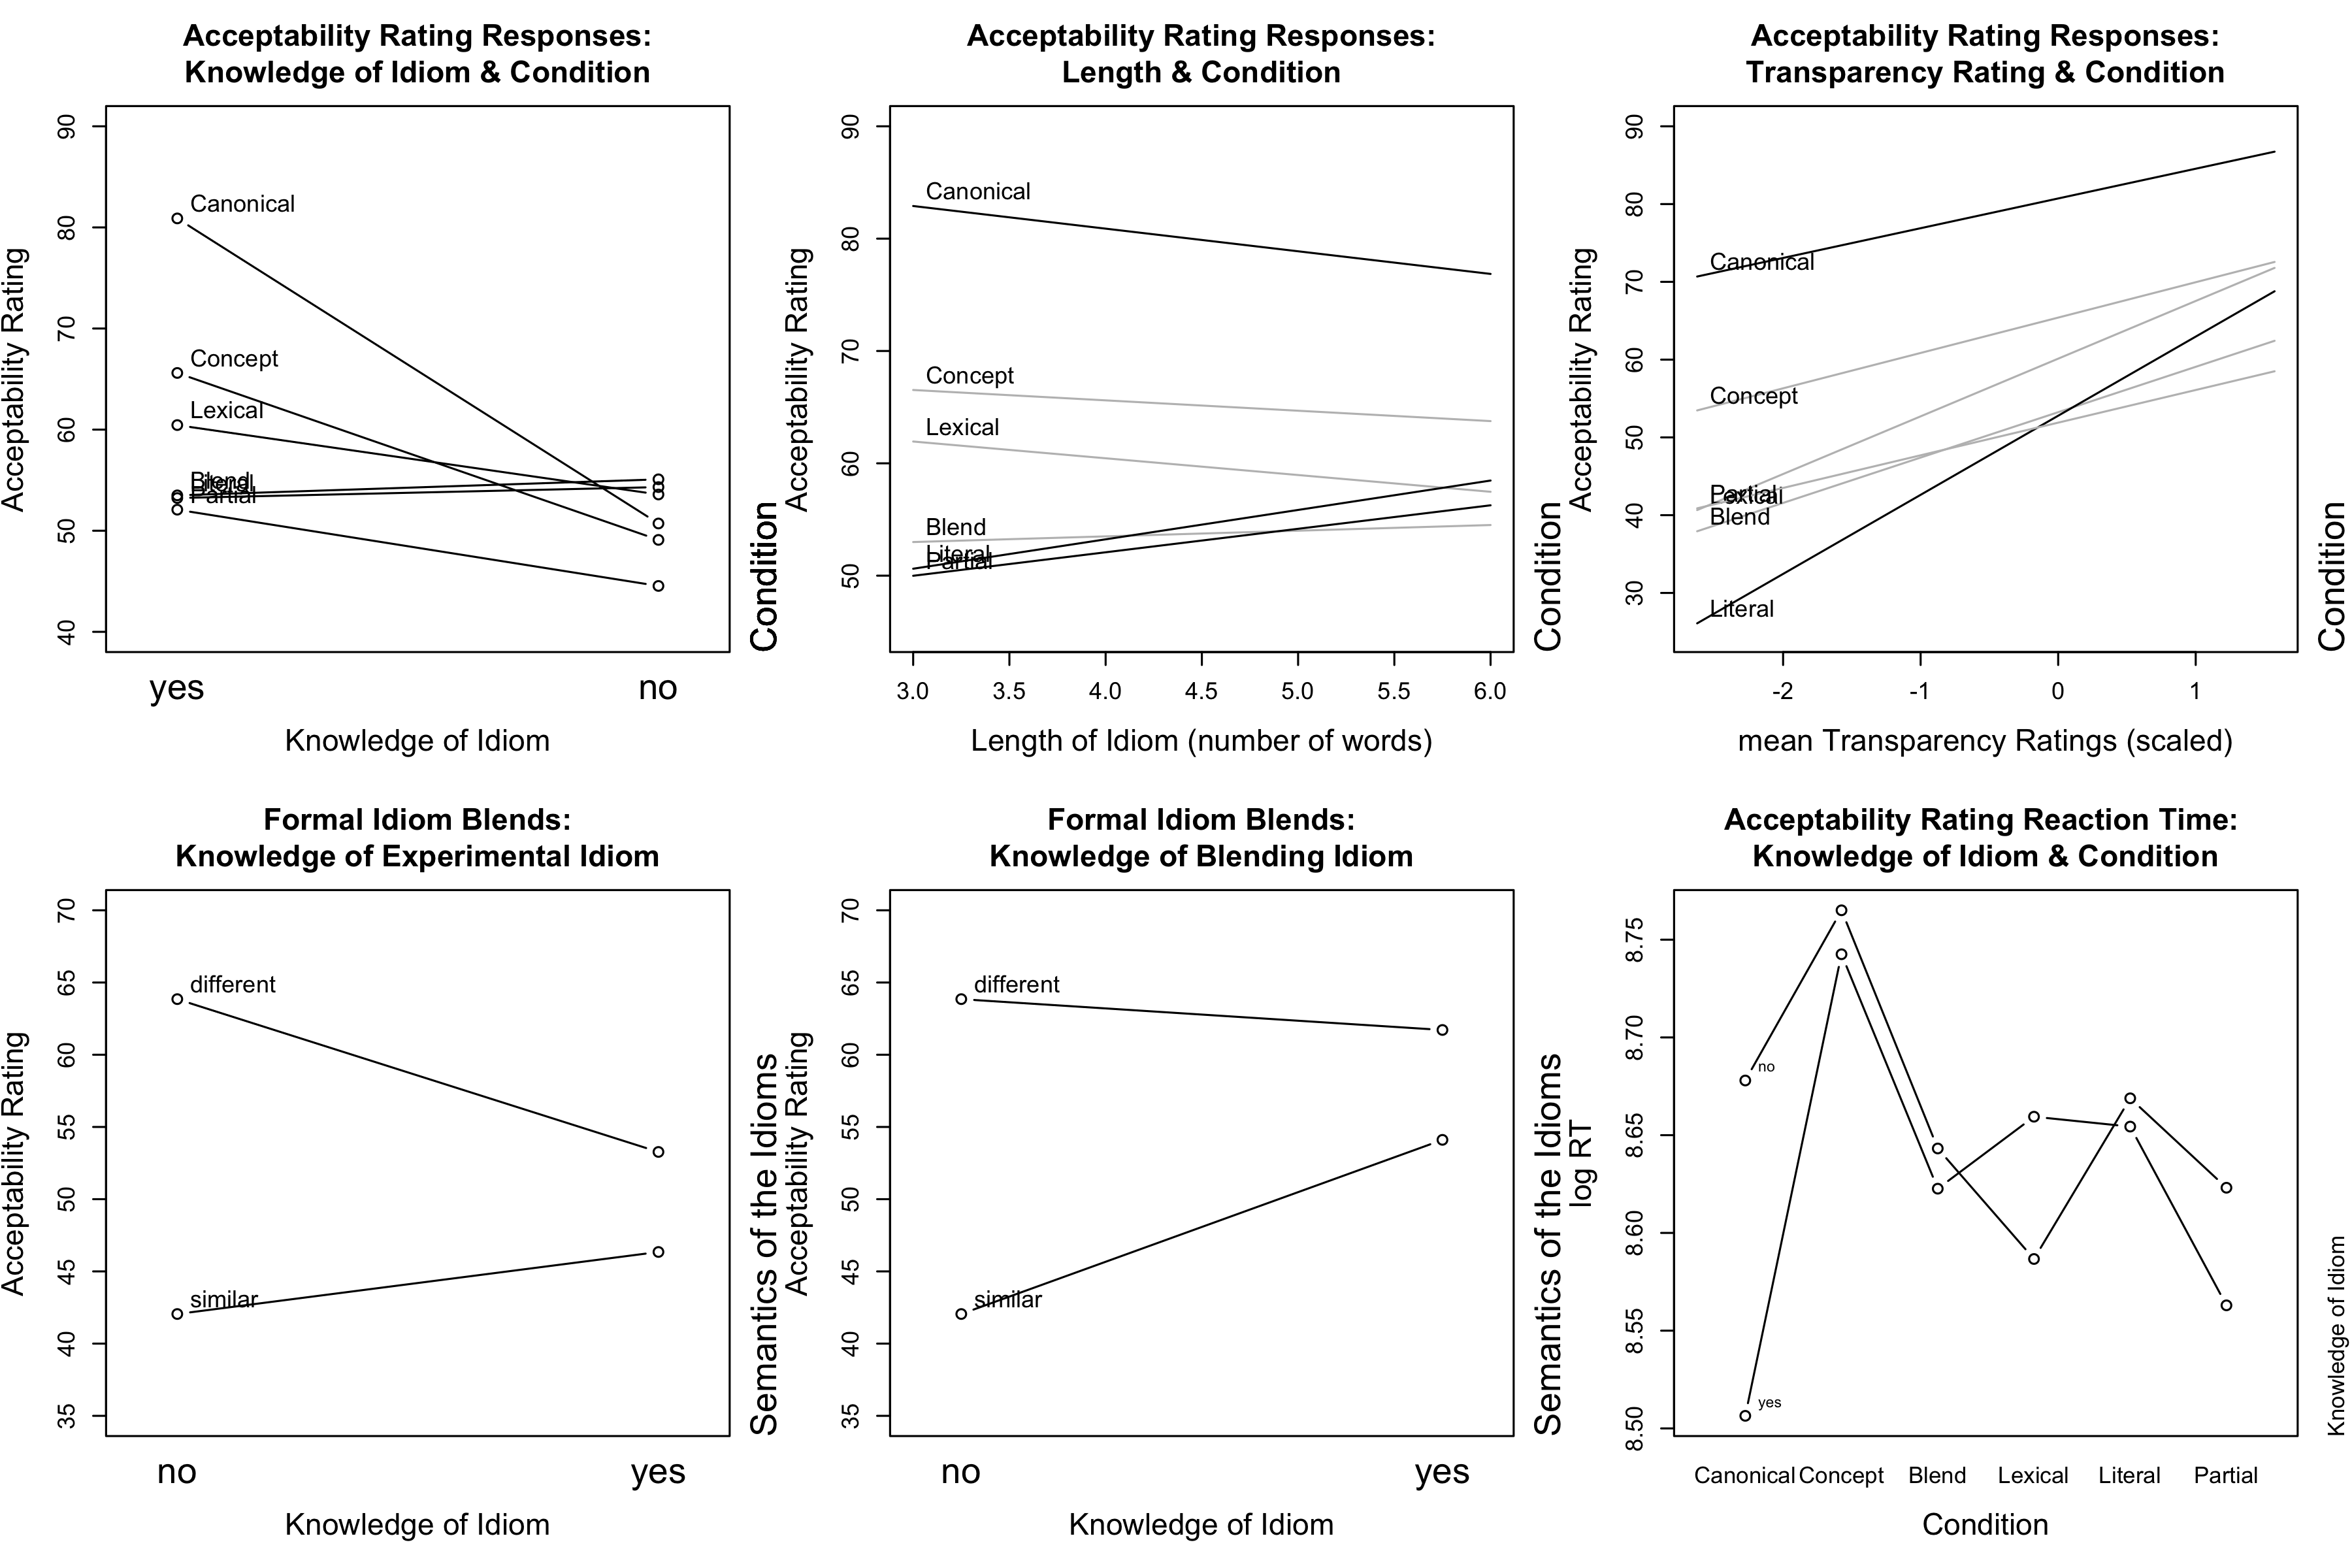
\includegraphics[width=\textwidth]{figures/ratings.png}
\caption{Interactions in the mixed-effects linear regression models for the acceptability rating responses and reaction times. Lines in grey represent factors levels which are not significantly different.}
\label{plotRatings}
\end{figure}

%\texttt{Trial} was significant as a main effect; participants became faster the further they advanced through the experiment. But participants differed in exactly how much faster they became, as evidenced by the by-Subject random slopes for \texttt{Trial}. 
\texttt{Trial} was significant as a main effect; participants became more accepting of the stimuli (both variants and the canonical form) the further they advanced through the experiment. But participants differed in exactly how much more accepting they became, as evidenced by the by-Subject random slopes for Trial. 
These slopes in the random effects structure are in addition to \texttt{Subject} and \texttt{Idiom} included as random effects.\footnote{The rating response model and the RT model show the same random effects structure.} Finally, it is interesting to note that the frequency or syntax of the idiom, as well as whether modifications were made to the verb or the noun, did not affect the acceptability\is{idiomatic variation!acceptability} of idioms\is{idiom} or variants. 

We also looked specifically at formal idiom\is{idiomatic variation!idiom blend} blends, given their error-like status in the literature \citep{Fay1982, CuttingBock1997}, in order to explore whether any factors influence their acceptability. Two interactions appear significant, shown in \tabref{NSblendsFixed}: both between the participant's knowledge of an idiom and the paired semantics of the two idioms involved in the blend. The bottom-left panel in \figref{plotRatings} shows the interaction with knowledge of the experimental idiom, while the bottom-centre panel shows the knowledge of the blending idiom. Both interactions indicate that blends are rated as more acceptable when the meanings of the two idioms differ, and less acceptable when they are similar. Participants significantly rate blends with similar semantics with a lower acceptability if one of the idioms is unknown. A three-way interaction between these variables (i.e. knowledge of both idioms and the semantic similarity of the idioms) is not significant, suggesting that speakers only need to be unfamiliar with one of the idioms to regard semantically similar idiom blends as less acceptable. The noticeability of the unknown idiom likely causes this increase in unacceptability, which is perhaps not as noticeable for those who are familiar with both blended idioms -- presumably, they are able to access the meaning of the blend easier, as they are familiar with both idioms from which the parts belong, and therefore are not as surprised or unimpressed by the blend. Finally, \texttt{meanTransparencyRating} is also significant in this model -- speakers prefer idiom blends that are more transparent\is{compositionality} and clearer in meaning. 



\begin{table}[ht]
\centering
\scriptsize{
\begin{tabular}{lrrrr}
\lsptoprule
 & Estimate & Std. Error & t-value & \textDelta  AIC\\ 
\midrule
Intercept & 63.62 & 6.06 & 10.50 &  \\ 
  meanTransparencyRating & 5.21 & 2.30 & 2.26 & 3.00 \\ 
  KnowExpIdiom=Yes & -10.58 & 4.64 & -2.28$^{*}$ & 1.02 \\ 
  KnowBlendingIdiom=Yes & -2.13 & 4.77 & -0.45 & 0.59 \\ 
  Semantics=Similar & -21.80 & 7.43 & -2.93$^{*}$ & 2.00 \\ 
  I(Semantics=Similar$|$KnowExpIdiom=Yes) & 14.87 & 6.47 & 2.30$^{*}$ & 3.23 \\ 
  I(Semantics=Similar$|$KnowBlendingIdiom=Yes) & 14.19 & 6.50 & 2.18$^{*}$ & 2.74 \\ 
\lspbottomrule
\end{tabular}
\ \\
$^{*}$ = Factors that remain significant after a Bonferroni correction\\
}
\caption{Fixed effects for the acceptability ratings of idiom blends.} 
\label{NSblendsFixed}
\end{table}




\subsubsection{Rating reaction times}

We also analyzed the \textsc{reaction times} (RTs) for how quickly the participants responded to the acceptability\is{idiomatic variation!acceptability} rating task. Faster reaction times are associated with easier judgements of acceptability. The fixed effects for this model are shown in \tabref{NSrtsFixed}. Only one interaction, between \texttt{KnowIdiom} and \texttt{Condition}, is significant in this model, illustrated in the bottom-right panel in \figref{plotRatings}. The RTs associated with each condition are similar for both those who know the idiom and those who do not. Significantly longer RTs are observed with integrated concepts, while significantly shorter RTs are observed with partial forms. These results may simply reflect the fact that the integrated concept\is{idiomatic variation!integrated concept}  condition has an additional word inserted into the idiom, whereas the partial form\is{idiomatic variation!partial form} condition has a word omitted from the expression. This RT difference likely corresponds to length of the expression. The most notable observation is that participants are significantly faster rating the canonical form of the expression if the idiom\is{idiom} is known. If the idiom is unknown, the RT to rate the canonical form does not differ significantly from the other variants. These results illustrate that the canonical form has an advantage if it is familiar, but that variants\is{idiomatic variation} of the same length as the canonical are rated as quickly as if one does not know the expression.\\ 


\begin{table}[ht]
\centering
\scriptsize{
\begin{tabular}{lrrrr}
\lsptoprule
 & Estimate & Std. Error & t-value & \textDelta AIC\\ 
\midrule
Intercept & 8.51 & 0.04 & 226.18 &  \\ 
  Condition=Concept & 0.24 & 0.02 & 9.65$^{*}$ & 93.85 \\ 
  Condition=Blend & 0.12 & 0.02 & 4.70$^{*}$ &  \\ 
  Condition=Lexical & 0.15 & 0.02 & 6.22$^{*}$ &  \\ 
  Condition=Literal & 0.15 & 0.02 & 5.92$^{*}$ &  \\ 
  Condition=Partial & 0.06 & 0.02 & 2.27 &  \\ 
  KnowIdiom=No & 0.17 & 0.04 & 4.40$^{*}$ & 1.69 \\ 
  Trial & -0.08 & 0.01 & -8.16 & 39.96 \\ 
  I(KnowIdiom=No$|$Condition=Concept) & -0.15 & 0.05 & -2.82$^{*}$ & 13.10 \\ 
  I(KnowIdiom=No$|$Condition=Blend) & -0.15 & 0.05 & -2.91$^{*}$ &  \\ 
  I(KnowIdiom=No$|$Condition=Lexical) & -0.24 & 0.05 & -4.67$^{*}$ &  \\ 
  I(KnowIdiom=No$|$Condition=Literal) & -0.16 & 0.05 & -3.08$^{*}$ &  \\ 
  I(KnowIdiom=No$|$Condition=Partial) & -0.11 & 0.05 & -2.18 &  \\ 
\lspbottomrule
\end{tabular}
\ \\
$^{*}$ = Factors that remain significant after a Bonferroni correction\\
}
\caption{Fixed effects for the acceptability rating reaction times.} 
\label{NSrtsFixed}
\end{table}



In sum, this experiment explored the acceptability\is{idiomatic variation!acceptability} of idiomatic variation, using several types of variants. The canonical form is the most preferred and participants are quicker at rating this form, but only when the expression is known. Modifying an idiom\is{idiom} makes it less acceptable, but the decrease in acceptability varies according to the type of alternation -- integrating an additional element\is{idiomatic variation!integrated concept} (\textit{go through the investment roof}) or replacing a word with a near-synonym\is{idiomatic variation!lexical} (\textit{go through the ceiling}) were considered more acceptable variants. We now turn our attention to how these variants are understood.\is{idiomatic variation!comprehension}


%%%%%%%%%%%%



\section{Eye-tracking experiment}
\subsection{Methodology}

\subsubsection{Materials}
This experiment utilized the same materials as the previous experiment.


\subsubsection{Procedure}

This experiment used the Eye-Link 1000, desk-top mounted video-based eye-tracking\is{eye-tracking} device, manufactured by SR Research. The eye-tracker sampled the pupil location and size at a rate of 1000Hz, and was calibrated using a 9-point calibration grid. Calibration occurred at the beginning of the experiment, after the practice, and again after every 22 sentences, for a total of five blocks. The computer screen resolution was set to 1920 x 1080 pixels.

The stimuli were presented in two parts. Participants first saw the ``context clause'' (e.g., \textit{ Although these were new stocks,}), followed by the ``idiom clause'' (e.g. \textit{they suddenly went through the roof}.) on a separate screen. Each trial began with a fixation cross presented for 1,000 msec on the left side of a light-grey screen. Next, they saw the context clause, also on a light-grey background, in a bold, black, Courier New 30-point font. Every clause was displayed in full and fit on one line. To exit this screen, participants had to trigger an invisible boundary in the bottom right corner. A blank, light-grey screen was presented for 1,000 msec before the fixation cross preceding the idiom clause appeared. The sequence of screens for the idiom clause was identical to the context clause.\is{idiom} 

Ten percent of the stimuli were followed by a true/false comprehension\is{idiomatic variation!comprehension} question, which pertained to the immediately preceding sentence, and were presented randomly throughout the experiment. Participants pushed one of two buttons on a game controller to answer these questions, which were clearly labelled on the question screen. The experiment began with a practice session, which consisted of six practice sentences and three questions. These were the same for all participants, although their order varied. 

All participants had normal or corrected-to-normal vision. The right eye of each participant was tracked. Participants sat approximately 85cm from the computer screen, with the camera placed on the desk about 35cm in front of the computer screen. The participants sat in a sound-proof booth, while the experimenter sat outside the booth, running the experiment. The lights were kept on. The experiment was self-paced and took about 45 minutes to complete. Each participant was given an opportunity for a short break half-way through the experiment.

After the participants had completed the eye-tracking\is{eye-tracking} portion, they were asked to complete three additional tasks: (1) to indicate their knowledge of each expression; (2) to answer questions pertaining to their idiom\is{idiom} usage; and (3) to rate the acceptability of the seven prescriptively ``incorrect'' sentences (LQs). These tasks were identical to the ones in the acceptability\is{idiomatic variation!acceptability} rating experiment.



\subsubsection{Participants}

Sixty linguistics undergraduate students from the University of Alberta participated in this experiment. All were native speakers of English, and all were different participants than those who participated in the previous study. There were 43 female and 17 male participants, ranging from 17--29 years of age. All participants were reimbursed for their time with course credit.



\subsection{Results}

The results were analyzed using \isi{mixed-effects linear regression}. We focus on the total fixation duration (i.e. the total amount of time spent fixating on the \textsc{area of interest}, or AOI) within two AOIs: the idiom as a whole (i.e. the summed fixations on all words within the idiom) and the altered word within the idiom (i.e. the synonymous word in lexical variation\is{idiomatic variation!lexical}, the additional word in the integrated concept\is{idiomatic variation!integrated concept}, the semantically vague ``replacement" word in partial forms,\is{idiomatic variation!partial form} and the word from another idiom in the idiom blend).\is{idiomatic variation!idiom blend} As above, the analyses only include the 60 experimental idioms. %Further information about this study can be found in \citet{Geeraert2016}. 

Ten predictor variables appeared significant in the models. \texttt{Condition}, \texttt{Know Idiom}, \texttt{Length}, \texttt{meanTransparencyRating}, and \texttt{Trial} are the same variables used in the previous experiment. \texttt{Gender} is a factor specifying whether the participant is male or female. \texttt{PortionAltered} is a factor specifying which part of the idiom (i.e. beginning/verb or ending/noun) was manipulated in the variant. And \texttt{meanVariationRating} is a scaled mean measure of acceptability\is{idiomatic variation!acceptability} for a particular idiom with a each type of variation -- these averaged ratings were extracted from the previous experiment and included here to determine if participants' preferences influence their ease of comprehension\is{idiomatic variation!comprehension}.

Two measures reflecting the semantic contribution of the constituents were utilized in analyzing these results. \texttt{meanTransparencyRating} (described above) and \texttt{LSA.Score.Paraphrase}, which is a measure of similarity using \textsc{latent semantic analysis} (LSA), between the words in the idiom and its paraphrase (e.g., \textit{spill the beans} `reveal a secret'). This score was obtained from a pairwise comparison of two texts (i.e. an idiom and its paraphrase), which compares the local contexts in order to obtain a value of similarity \citep{LandauerEtAl1998}.\footnote{The LSA scores were obtained from the English Lexicon Project \citep{BalotaEtAl2007}, available at http://lsa.colorado.edu.} This measure allows us to control for the idiom's \isi{compositionality}. If the exact words in the idiom have little to do with the expression's meaning, then the LSA score will be small (e.g., \textit{cut the mustard} `be acceptable' = 0.07). But if the words used share meaning or contribute to the idiom's meaning, then the LSA score will be larger (e.g., \textit{stop something in its tracks} `stop something' = 0.87).
   
As idioms\is{idiom} are MWEs,\is{multiword expression} multiple frequency measures were obtained: the frequency of the idiom, frequencies of the individual words, and all possible combinations of adjacent words (e.g. word1 and word2; word2 and word3; word1 and word2 and word3). To avoid collinearity, a \textsc{principal components analysis} (PCA) was conducted on these frequency measures. Only the first principal component (henceforth \texttt{PC1.logFrequency}) is significant. Finally, a second PCA was conducted on the rating responses for the seven LQs above. Only PC2 (henceforth \texttt{PC2.LQ}) was significant. This latent variable may reflect the participant's flexibility with language usage.


\subsubsection{Idiom as AOI}

The first model examines the summed fixation durations on the idiom as a whole. The fixed effects for this model are shown in \tabref{idiomTFDfixed}. The first interaction, between \texttt{Condition} and \texttt{KnowIdiom}, is shown in the left panel of \figref{plotEyetracking}. The canonical form, and the majority of variants, show the same general pattern: shorter fixation durations on known idioms\is{idiom}. These variants (except integrated\is{idiomatic variation!integrated concept} concepts) are therefore shown in grey, as they do not significantly differ from the canonical form. Partial forms\is{idiomatic variation!partial form} however show a different pattern. Fixation durations are relatively similar regardless of whether the participant is familiar with the expression or not; thus a facilitation effect for knowing the idiom is not observed as it is with the other variants. This particular variant is fixated upon less than the canonical form, likely due to it being shorter in length (i.e. fewer number of words). This is in line with longer fixations observed on integrated concepts -- an additional word is integrated into the idiom, making it longer in length and requiring additional fixations.\is{idiomatic variation!comprehension}


\begin{table}[ht]
\centering
  \scriptsize{
\begin{tabular}{lrrrr}
\lsptoprule
 & Estimate & Std. Error & t-value & \textDelta  AIC\\ 
\midrule
Intercept & 6.71 & 0.09 & 75.97 &  \\ 
  Condition=Concept & 0.49 & 0.10 & 5.04$^{*}$ & 130.12 \\ 
  Condition=Blend & 0.08 & 0.10 & 0.75 &  \\ 
  Condition=Lexical & 0.01 & 0.10 & 0.05 &  \\ 
  Condition=Literal & -0.19 & 0.10 & -1.94 &  \\ 
  Condition=Partial & -0.75 & 0.16 & -4.80$^{*}$ &  \\ 
  KnowIdiom=Yes & -0.18 & 0.04 & -4.32$^{*}$ & 34.84 \\ 
  Length & 0.11 & 0.02 & 6.76 & 40.19 \\ 
  PortionIdiomAltered=Ending & -0.06 & 0.02 & -2.52$^{*}$ & 3.50 \\ 
  PC2.LQ & -0.07 & 0.03 & -2.42 & 3.60 \\ 
  LSA.Score.Paraphrase & 0.24 & 0.07 & 3.49 & 8.21 \\ 
  meanVariationRating & -0.06 & 0.01 & -7.23 & 43.80 \\ 
  Gender=Male & -0.17 & 0.08 & -2.17 & 2.53 \\ 
  TrialScaled & -0.04 & 0.01 & -3.78 & 10.80 \\ 
  I(KnowIdiom=Yes$|$Condition=Concept) & 0.06 & 0.05 & 1.16 & 1.26 \\ 
  I(KnowIdiom=Yes$|$Condition=Blend) & 0.08 & 0.06 & 1.42 &  \\ 
  I(KnowIdiom=Yes$|$Condition=Lexical) & 0.08 & 0.06 & 1.52 &  \\ 
  I(KnowIdiom=Yes$|$Condition=Literal) & 0.03 & 0.06 & 0.55 &  \\ 
  I(KnowIdiom=Yes$|$Condition=Partial) & 0.17 & 0.06 & 2.75$^{*}$ &  \\ 
  I(Length$|$Condition=Concept) & -0.05 & 0.02 & -2.62 & 14.11 \\ 
  I(Length$|$Condition=Blend) & -0.01 & 0.02 & -0.36 &  \\ 
  I(Length$|$Condition=Lexical) & 0.00 & 0.02 & 0.20 &  \\ 
  I(Length$|$Condition=Literal) & 0.02 & 0.02 & 1.04 &  \\ 
  I(Length$|$Condition=Partial) & 0.08 & 0.03 & 2.48 &  \\ 
\lspbottomrule
\end{tabular}
\ \\
$^{*}$ = Factors that remain significant after a Bonferroni correction\\
   }
\caption{Fixed effects for the idiom as AOI.} 
\label{idiomTFDfixed}
\end{table}


The second interaction, shown in the second panel of \figref{plotEyetracking}\is{eye-tracking}, is between \texttt{Condition} and \texttt{Length}. Longer idioms show longer summed fixation durations, as expected, due to the increased number of words in the idiom. Lexical\is{idiomatic variation!lexical} variation, formal idiom\is{idiomatic variation!idiom blend} blends, and the \isi{literal meaning} of the idiom are not significantly different from the canonical form (shown in grey). The other two variants show a pattern that is significantly different from the canonical form. Integrated concepts show a slight inhibitory effect of length, where an additional concept is more difficult to integrate into shorter idioms (i.e. extra time is required). Whereas partial forms of shorter idioms have even fewer words to fixate upon and therefore show considerably shorter fixation durations. Thus, durations on integrated concepts\is{idiomatic variation!integrated concept} and partial forms\is{idiomatic variation!partial form} are more comparable to the canonical form when the idiom is longer.\footnote{\texttt{PC1.logFrequency} was also significant in the idiom as AOI model. However, this variable is strongly correlated with \texttt{Length} (\textit{r} = -0.9). This correlation is unsurprising given that \texttt{PC1.logFrequency} was created using adjacent co-occurrence frequencies. Model comparison shows that \texttt{Length} is the more significant predictor in this model, producing a considerably lower AIC value, and therefore was retained at the expense of \texttt{PC1.logFrequency}.}\is{idiomatic variation!comprehension}

Interestingly, the literal meaning of the idiom shows shorter fixation durations than the canonical form, albeit not quite significantly shorter (\textit{t} = -1.94). The literality of the expression \citep{TitoneConnine1994b} may be contributing to this result. Nevertheless, a general pattern is evident based on these two above interactions with \texttt{Condition}: variants of the same length as the canonical form are not processed significantly different from this canonical form.


\begin{figure}
\centering
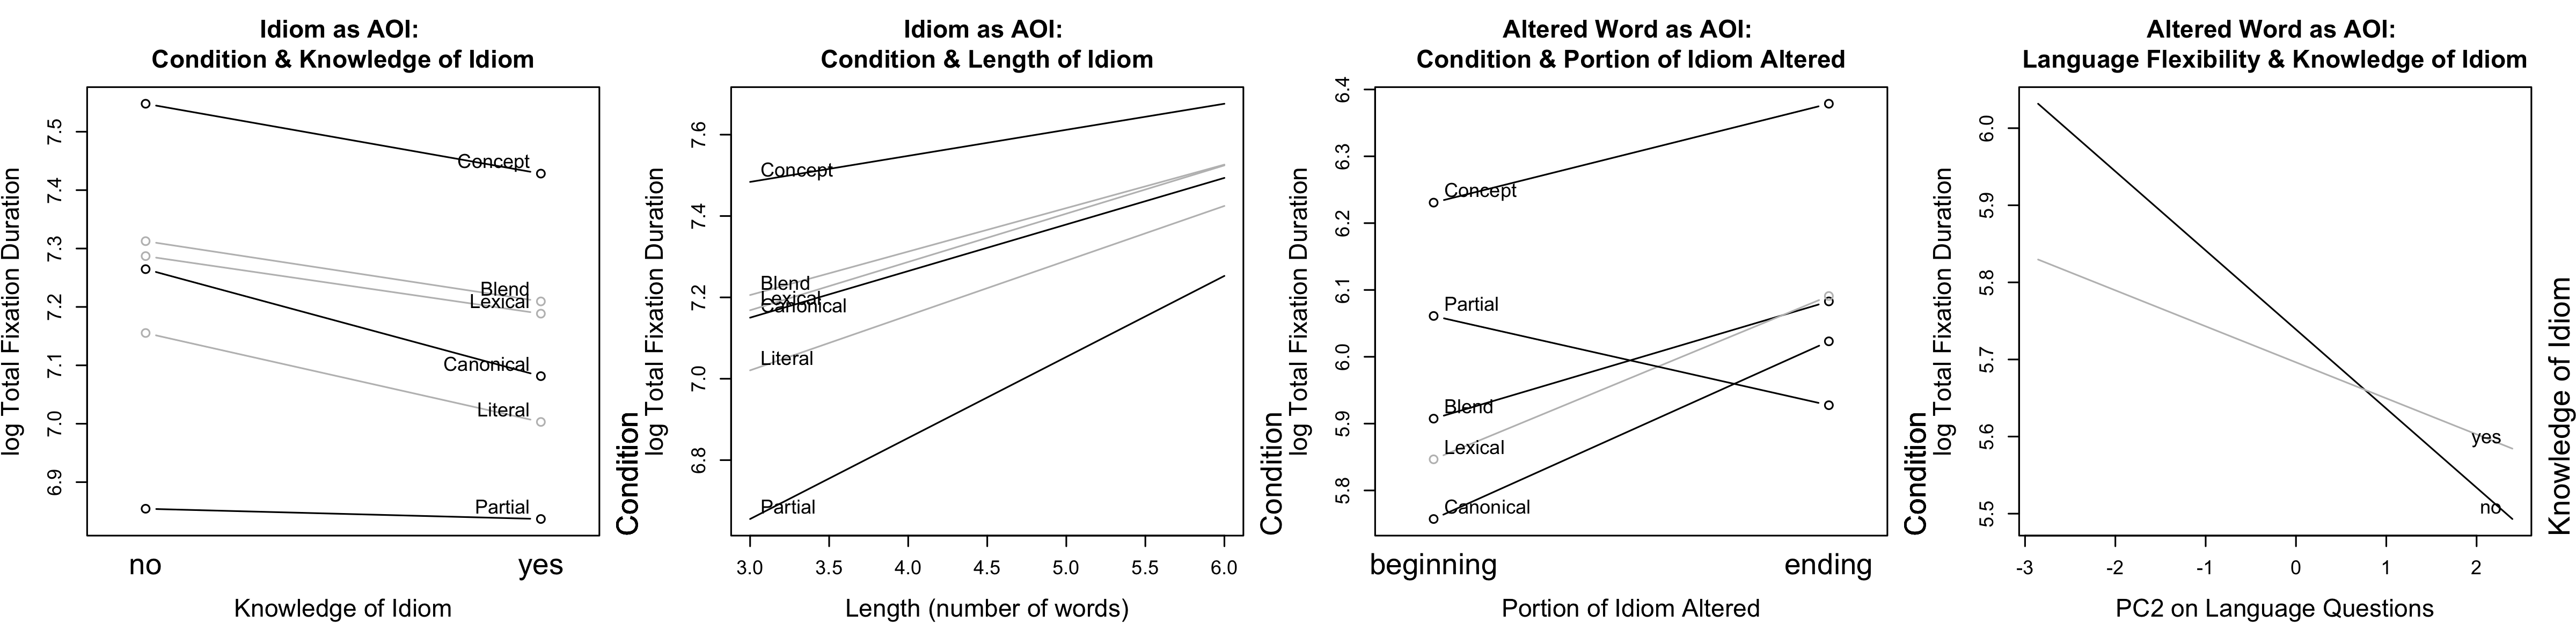
\includegraphics[width=\textwidth]{figures/eyetracking.png}
\caption{Interactions in the mixed-effects linear regression models for the summed total fixation duration on the whole idiom and the altered word as an AOI. Lines in grey represent factor levels which are not significantly different or slopes which are not significant.}
\label{plotEyetracking}
\end{figure}


%The literal meaning is also associated with an increased number of comprehension questions answered incorrectly (X = 63.75; \textit{p} = 0). Two possibilities might explain this outcome. First, participants may have needed additional time processing the literal meaning -- a duration more comparable with the canonical form -- to fully integrate the literal meaning of the idiom into the preceding context. Hence, they could have gotten the comprehension questions wrong because they read the idiom too quickly. Second, the `literality' (i.e. the degree to which an idiomatic phrase has a plausible literal interpretation) of the idioms used in these questions was not controlled for, and some idioms, such as \textit{have a card up your sleeve}, elicit higher ratings for literality than idioms like \textit{foot the bill} \cite{TitoneConnine:1994b,TitoneConnine:1994a}. It is likely that the questions for idioms associated with a lower literality rating brought the overall correctness down for this condition.



Six main effects are observed in this model. Longer fixation durations are observed on the whole idiom\is{idiom} if the beginning (the verb) was altered (i.e. \texttt{Portion Altered}). This is not dependent on the type of variation; all variants are easier to process\is{idiomatic variation!comprehension} if the change comes later in the idiom. This is a different result than that of Gibbs and colleagues \citep{GibbsEtAl1989, GibbsNayak1989} who found no difference with similarity ratings in whether the noun or verb was altered. %(note the absence of an effect with the acceptability ratings).

\texttt{MeanVariationRating} is also significant. Variants which received higher acceptability\is{idiomatic variation!acceptability} ratings are fixated on less long, suggesting preferred variants are easier to understand and interpret (or perhaps variants easier to interpret are preferred). Longer fixation durations appear on idioms\is{idiom} which have higher LSA scores for the idiom's paraphrase (i.e. \texttt{LSA.Score.Paraphrase}). This finding seems initially surprising, as previous analyses on the comprehension\is{idiomatic variation!comprehension} of idioms suggest that idioms are easier to understand when the individual components contribute meaning\is{compositionality} to the whole \citep{GibbsEtAl1989}. However, the LSA scores indicate how similar the local contexts are between the idiom and its paraphrase (i.e. how interchangable is the idiom and its paraphrase). When the LSA score is high (i.e. the paraphrase is easily interchangable), looking time increases as the contexts are not distinctive for the idiom. But if the LSA score is low, then the idiom and its paraphrase are less interchangable, making the context more distinctive and the idiom more predictable.\is{predictability} Interestingly, \texttt{meanTransparencyRating} is not significant. The degree to which the idiom is considered obvious in meaning does not seem to influence the comprehension\is{idiomatic variation!comprehension} of idioms or variants. %only its acceptability.

A main effect is also observed for \texttt{PC2.LQ}, a latent variable representing the participants' ``flexibility" with language (i.e. the more they consider nonstandard or erroneous forms acceptable).\is{idiomatic variation!acceptability} Shorter fixations are observed on idioms\is{idiom}, both the canonical form and variants, if speakers are more flexible with language. It is interesting to note that this finding is not  restricted to only the variants. \texttt{Gender} also shows a significant main effect -- males tend to fixate less long on the idiom than females, although we are not quite sure why. Finally, a main effect of \texttt{Trial} is also significant; participants fixate less long on the idiom the further into the experiment they get. But the degree to which each participant is affected by the order of presentation varies, as evidenced by significant by-Subject random slopes for \texttt{Trial}.\footnote{Both idiom as AOI and altered word as AOI models have the same random effects structure.} By-Item random slopes for \texttt{Condition} with correlation parameters are also significant in this model. These slopes indicate that participants' fixation durations vary depending on which idiom occurred in which condition -- participants found certain idioms easier or more difficult to understand\is{idiomatic variation!comprehension} depending on the condition in which they occurred. 



\subsubsection{Altered word as AOI}

We next investigate the fixation duration on the altered word (i.e. the word in the idiom that was manipulated). The fixed effects for this model are shown in \tabref{MwordTFDfixed}. As there is no altered word in the literal condition, this section focuses on the four idiom variants: lexical variation, partial forms, idiom\is{idiomatic variation!idiom blend} blends, and integrated\is{idiomatic variation!integrated concept} concepts, and how they compare to the canonical form. 

The interaction between \texttt{Condition} and \texttt{PortionAltered} is seen in the third panel of \figref{plotEyetracking}\is{eye-tracking}. The overall pattern is that longer fixation durations occur at the end of the idiom, which is also true for the canonical form. Since the idiom occurs at the end of a sentence, these longer fixations may reflect a sentence wrap-up effect \citep{RaynerEtAl2000, HirotaniEtAl2006}. Nevertheless, the altered word for most variants shows significantly longer fixations than the canonical form. This is not true of lexical variation\is{idiomatic variation!lexical}, which is the only variant that does not have significantly longer fixations than the canonical form (\textit{t} = 1.54). Thus, a lexically altered variant is just as easy to process\is{idiomatic variation!comprehension} as the canonical form. Partial forms\is{idiomatic variation!partial form} however, appear considerably different from the canonical form. Longer fixations are observed on the altered word when the beginning has been altered, as in \textit{use the grapevine}. But when the ending is altered (e.g., \textit{spilled it}), fixations on the altered word are not significantly different from the canonical form (\textit{t} = -1.44). 
%Altering the verb does not always result in significantly longer fixations (cf. the non-significantly different lexical variant when the beginning is altered), therefore this finding suggests that altering the verb to a semantically vague verb  (i.e. \ile{be}, \ile{do}, \ile{used} -- in order to make the sentence grammatical), significantly inhibits processing.
Altering the verb does not always result in significantly longer fixations (cf. the non-significantly different lexical variant when the beginning is altered),
however altering the verb to a semantically vague verb (i.e. \ile{be}, \ile{do}, \ile{used} – in order to make the sentence grammatical) does significantly inhibit processing.

\begin{table}[htb]
\centering
  \scriptsize{
\begin{tabular}{lrrrr}
\lsptoprule
 & Estimate & Std. Error & t-value & \textDelta  AIC \\
\midrule
Intercept & 5.70 & 0.06 & 98.48 &  \\ 
  Condition=Concept & 0.47 & 0.06 & 8.28$^{*}$ & 58.40 \\ 
  Condition=Blend & 0.15 & 0.06 & 2.67$^{*}$ &  \\ 
  Condition=Lexical & 0.09 & 0.06 & 1.54 &  \\ 
  Condition=Partial & 0.30 & 0.07 & 4.61$^{*}$ &  \\ 
  PortionIdiomAltered=Ending & 0.27 & 0.06 & 4.49$^{*}$ & 17.88 \\ 
  KnowIdiom=Yes & -0.04 & 0.03 & -1.29 & 0.21 \\ 
  PC2.LQ & -0.10 & 0.03 & -3.12 & 2.59 \\ 
  PC1.logFrequency & 0.03 & 0.01 & 4.70 & 15.43 \\ 
  meanVariationRating & -0.07 & 0.02 & -4.27 & 14.09 \\ 
  TrialScaled & -0.04 & 0.01 & -2.79 & 5.28 \\ 
  I(PortionIdiomAltered=Ending$|$Condition=Concept) & -0.12 & 0.08 & -1.46 & 9.81 \\ 
  I(PortionIdiomAltered=Ending$|$Condition=Blend) & -0.09 & 0.08 & -1.17 &  \\ 
  I(PortionIdiomAltered=Ending$|$Condition=Lexical) & -0.02 & 0.08 & -0.26 &  \\ 
  I(PortionIdiomAltered=Ending$|$Condition=Partial) & -0.40 & 0.09 & -4.42$^{*}$ &  \\ 
  I(PC2.LQ$|$KnowIdiom=Yes) & 0.06 & 0.02 & 2.27$^{*}$ & 3.09 \\ 
\lspbottomrule
\end{tabular} 
\ \\
$^{*}$ = Factors that remain significant after a Bonferroni correction\\
}
\caption{Fixed effects for the altered word as AOI.}
\label{MwordTFDfixed}
\end{table}
 

The second interaction, shown in the last panel of \figref{plotEyetracking}\is{eye-tracking}, is between knowledge of the idiom\is{idiom} (i.e. \texttt{KnowIdiom}) and the participant's flexibility with language (i.e. \texttt{PC2.LQ}). Flexibility with language only appears facilitative for those who do not know the idiom, illustrated by the non-significant slope (in grey) for those who know the expression. Other strategies are apparently relied upon to interpret the idiom when knowledge of it is not available. 

Additional main effects are also observed. Fixation durations are longer on the altered word when the co-occurrence frequencies of the idiom are higher. Thus, altering part of a more frequent sequence causes greater processing costs. In addition, participants have shorter fixation durations when the variant is rated as more acceptable (i.e. \texttt{meanVariationRating}). The more the variation strategy\is{idiomatic variation} is preferred with a particular idiom, the easier it is to interpret. Finally, the further the participants get into the experiment (i.e. \texttt{Trial}), the shorter their fixation durations on the altered word. 

We also specifically looked at idioms blends,\is{idiomatic variation!idiom blend} to determine whether the syntax or the semantics of the two merged idioms affects the processing of this variant. Interestingly, neither of these variables were predictive of fixation duration -- we can understand\is{idiomatic variation!comprehension} idiom blends regardless of the syntax or the semantics of the two idioms used in the blend.



%\subsection{Spillover from the Altered Word}

Some of these alternations may have been surprising to the participants, resulting in effects that continued beyond the altered word. We therefore ran a model to explore any spillover effects from the altered word, shown in \tabref{surWordTFDfixed}. As the idiom\is{idiom} occurred in sentence-final position, spillover effects from an altered noun (i.e. the end of the idiom) are not able to be determined; thus, this model only focuses on spillover effects from an altered verb. We examined the fixation duration on the first content word after the verb when the verb was manipulated (i.e. the alternation occurred at the beginning of the idiom).  


\begin{table}[ht]
\centering
  \scriptsize{
\begin{tabular}{lrrrr}
\lsptoprule
 & Estimate & Std. Error & t-value & \textDelta  AIC\\ 
\midrule
Intercept & 5.95 & 0.08 & 73.41 &  \\ 
  Condition=Concept & 0.27 & 0.07 & 3.76$^{*}$ & 11.6 \\ 
  Condition=Blend & 0.17 & 0.06 & 2.75$^{*}$ &  \\ 
  Condition=Lexical & 0.14 & 0.05 & 2.92$^{*}$ &  \\ 
  Condition=Partial & 0.30 & 0.06 & 4.62$^{*}$ &  \\ 
  PC1.logFrequency & 0.04 & 0.01 & 3.54 & 6.38 \\ 
  KnowIdiom=Yes & -0.11 & 0.05 & -2.32$^{*}$ & 3.20 \\ 
\lspbottomrule
\end{tabular}
\ \\
$^{*}$ = Factors that remain significant after a Bonferroni correction\\
}
\caption{Fixed effects for the first content word after the verb.} 
\label{surWordTFDfixed}
\end{table}


Spillover effects are observed for all variant types (i.e. \texttt{Condition}), but the longest durations are for integrated concepts\is{idiomatic variation!integrated concept} and partial\is{idiomatic variation!partial form} forms. Incorporating an additional word into an idiom results in a processing cost likely due to the surprisal of this extra word. Integrating this additional information into the idiom and context requires extra time. The largest spillover effect is with partial forms. It appears that the semantically vague words used in these sentences (to make them grammatical) make these partial forms more difficult to comprehend\is{idiomatic variation!comprehension} and cause considerable spillover effects. It remains to be determined whether partial forms from more naturalistic language produce this same effect.

The last two effects are \texttt{PC1.Frequency} and \texttt{KnowIdiom}. The higher the co-occurrence frequencies of the idiom, the longer the fixation duration on the first content word after the alternation. Modifying a frequent multiword sequence\is{multiword expression} inhibits processing. However, these spillover effects are reduced if the idiom\is{idiom} is familiar (i.e. \texttt{KnowIdiom}).  


%However, for variants in which the beginning portion of the idiom was altered (the verb), it may appear to the participant reading the text as though the ending was manipulated (e.g. as if the `blending idiom' was the intended idiom in \textit{call the strings}, or part of an idiom was inserted into an otherwise non-idiomatic text, such as \textit{use the grapevine})



%%%%%%%%%%%%

\section{Discussion} 

This study employed a multi-methodological  approach to investigate the acceptability\is{idiomatic variation!acceptability} and processing\is{idiomatic variation!comprehension} of \isi{idiomatic variation}. One advantage of using multiple methods is that they can reveal greater insights, by contrasting converging and diverging results between the different methods. Converging results can provide greater confidence that a particular result or predictor variable is robust; whereas diverging results can uncover differences due to a specific modality or shed light on findings concerning the larger picture that would otherwise be overlooked or thought contradictory \citep{ArppeJarvikivi2007}. The findings between the acceptability rating and eye-tracking\is{eye-tracking} experiments presented together in this chapter do in fact show converging and diverging results  worthy of discussion.

Interestingly, the findings between the experiments primarily show diverging results with regard to our two research questions. For example, our first research question asks how the variants compare with the canonical form, and we see from the acceptability ratings that the canonical form is rated as more acceptable than variants or a literal reading, with speakers clearly preferring this form. However, the processing differences are not nearly as straightforward. Some variants are processed\is{idiomatic variation!comprehension} differently than the canonical form. The variant showing the greatest difference from the canonical form is the partial form\is{idiomatic variation!partial form} of the idiom (e.g., \textit{use the grapevine}). This idiom\is{idiom} variant\is{idiomatic variation} is fixated on less than the canonical form, as expected, largely due to the omission of a word (or words) from the expression. Yet despite this shorter fixation on the whole idiom, participants fixated significantly longer on the ``replacement'' verbs (i.e. the semantically vague verbs used to connect the idiom to the sentence) and significant spillover effects were observed on the first content word after these verbs. A similar inhibitory effect was not observed if the ending was modified (e.g., \textit{spilled it}). These results are likely due to the design of the experiment. The tightly controlled stimuli used in this study made these partial forms unnatural and difficult to interpret. A study investigating partial forms in naturally occurring language may shed more light on the degree of difficulty for processing this variant.

Idioms\is{idiom} with additional concepts integrated\is{idiomatic variation!integrated concept} into the expression are also processed differently from the canonical form. These variants require additional processing\is{idiomatic variation!comprehension} time, as anticipated, but this longer reading time is largely attributable to the extra word in the expression. The longer duration on the whole idiom is very similar to the altered word AOI, suggesting that this variant experiences very little processing costs over and above having to read an extra word.
 
However, modification of an idiom's form does not always result in a processing disadvantage. Some variants -- lexical variation\is{idiomatic variation!lexical}, formal idiom\is{idiomatic variation!idiom blend} blends, and a literal\is{literal meaning} reading of the idiom -- are not processed significantly slower than the canonical. Differences between these variants and the canonical form are observed, such as longer fixations on the altered word (at least for idiom blends) or some spillover effects if the verb was altered, but these differences do not result in longer reading times for the idiom as a whole. These findings are partly in line with our predictions. Only idiom blends were predicted to be processed slower than the canonical form, due to the potential surprisal at or unrecognizability with this so-called error. But as observed, they do not present difficulties in comprehension\is{idiomatic variation!comprehension}. Thus, intentional or not, altering a word within an idiom to a synonymous or non-synonymous word does not result in a processing cost.

Our second research question asks how variants compare with each other. Once again, diverging results between the two methods are evident.  Lexical variation and idiom blends are processed quite similarly, showing comparable fixation durations, to each other and to the canonical form. The length of the original idiom is maintained in these variants, possibly explaining these comparable durations. However, they do not share similar acceptabilities.\is{idiomatic variation!acceptability} Lexically modified variants\is{idiomatic variation!lexical} are considered much more acceptable than idiom blends. In fact, idiom blends\is{idiomatic variation!idiom blend} are even less preferred when the two idioms used to make the blend share similar semantics, possibly explaining why blends are often viewed as errors \citep{Fay1982, CuttingBock1997}. Meanwhile, integrated concepts,\is{idiomatic variation!integrated concept} which add extra information into the idiom, show longer reading times than the other variants, yet are the most preferred. This higher acceptability was expected, given their relatively frequent occurrence in corpora \citep{Moon1998, Schroder2013}, and leaves us wondering whether semantically productive lexical variants \citep[cf.][]{McGloneEtAl1994} would show higher levels of acceptability (on par with integrated concepts) compared with the synonymous lexical variants utilized here \citep[following][]{GibbsEtAl1989}. Finally, partial forms\is{idiomatic variation!partial form} and a literal reading of the idiom are not acceptable variation strategies, even though they have comparable (or shorter) reading times to the canonical form.

The findings from these two research questions present two main observations. First, variants\is{idiomatic variation} which add an extra element or are truncated in some way show longer or shorter reading times, respectively, while modifications that maintain the same length as the canonical form show comparable reading times to the canonical form. Second, variants that preserve more of the canonical form (e.g. integrated concepts, lexical variation) are considered more acceptable, although preference remains with the canonical form (which likely facilitates the learning of idioms\is{idiom} and leads to faster recognition).

One cautionary note must be made. These aggregated results show patterns and preferences, but they do not imply that all idioms can be altered using all variation strategies. Much variability, particularly when it comes to comprehension\is{idiomatic variation!comprehension}, is also observed. Including the mean acceptability\is{idiomatic variation!acceptability} for each idiom in each condition as a control variable in the comprehension models resulted in preferred variants showing shorter reading times. In other words, the way in which an idiom is modified can affect how easy it is to understand. Variability is also observed in the random effects structure of the comprehension models, which have by-Item random slopes with correlation parameters for \texttt{Condition}, indicating that specific idioms can be easier or more difficult to process depending with which condition they occurred. Thus, while variation\is{idiomatic variation} is possible and general patterns can be observed, there are also idiom-specific preferences that factor into how an idiom is altered, understood, and appreciated. 

   
% Literal - one of the least preferred variants, but more accepting if longer (more words to infer...) and if the idiom is seen as more transparent. Speakers do not like a literal interpretation with the canonical form - evidence that shows a literal reading is used differently (Moon 1998 - break ice, break ice into, break the ice with, the ice breaks -- different distributions for literal meaning). But still able to be understood, similar to canonical


Converging and diverging results  are also observed with the predictor variables in the analyses. Two variables converge between the two methods. Length is shown to be an important predictor and yet is rarely included in the idiom literature \citep[cf.][]{FanariEtAl2010}. Longer idioms\is{idiom} require additional processing time, as expected, and there can be some facilitation or inhibitory processing effects depending on the type of variation encountered. A literal reading gains additional approval when the idiom is longer (and perhaps also more transparent), while shorter idioms are even more preferred with the idiomatic reading. Perhaps the extra words in longer idioms clearly identify the metaphorical links associated with the idiom, making a literal reading\is{literal meaning} also more interpretable.

The participant's knowledge of the expression is another important predictor that converges between the two studies.  Participants fixated less on the idiom (i.e. shorter reading times) and were faster to rate the expression when they knew the idiom. They also considered the idiom and its variants as more acceptable when it was familiar. Yet surprisingly, research on idioms\is{idiom} tends to include an average measure of familiarity \citep[cf.][]{TitoneConnine1994}, as a control for frequency or as a measure of subjective familiarity. This study demonstrates that a speaker-specific measure of familiarity is important for idiom research, as it incorporates speaker-specific experiences into the model.

Not all participant-related variables show converging results. The language questions (LQs) that were collected to provide a latent measure of the participant's flexibility with language only appeared significant in predicting the comprehension\is{idiomatic variation!comprehension} of idioms, and not their acceptability\is{idiomatic variation!acceptability}. Participants who are more flexible (i.e. more accepting of non-standard or erroneous forms) have an easier time processing idioms and variants. This of course makes sense; these speakers are not distracted by the specific form used, but focus solely on the message being conveyed.  

Frequency was also not predictive of acceptability\is{idiomatic variation!acceptability}. Even highly frequent idioms can be regarded as acceptable when altered. But frequency is predictive of comprehension\is{idiomatic variation!comprehension}. This variable only appeared in the altered word model (due to the high correlation with length in the idiom model), and revealed that alternations made to frequent idioms result in a processing cost. When a sequence of words that typically occur together has been modified, additional time is required to interpret the new sequence, as the advantage it once received due to its \isi{predictability} is no longer available. The opposite pattern is observed for the semantics of formal idiom blends\is{idiomatic variation!idiom blend} -- a significant predictor of acceptability, but not comprehension. Speakers find blends unacceptable when the merged idioms share similar semantics, but appear to have no difficulty interpreting them.

A divergence is also seen with the variable \texttt{PortionAltered} (i.e. where in the idiom the alternation occurred: beginning/verb or ending/noun). This variable is not predictive of acceptability -- participants' judgements were not affected by where in the idiom the alternation occurred (i.e. modifications to nouns and verbs are equally acceptable). However, this variable is predictive of comprehension -- alternations made earlier in the idiom (the verb) result in greater processing costs. \citet{GibbsEtAl1989} found no difference between modifications made to nouns or verbs in their similarity rating task, providing further confirmation that a subjective rating of similarity is not measuring comprehension\is{idiomatic variation!comprehension}. In addition, these results may also provide support for a time-dependent nature of idiom processing \citep{TitoneLibben2014}. As one advances through the idiom, the \isi{predictability} of the idiom becomes greater and the idiomatic meaning accumulates resulting in greater priming effects for later words. It seems reasonable then that changes made later in the expression will be less costly -- the meaning is more predictable even if changes have been made.

Finally, a divergence is also evident between which \isi{compositionality} measure was determined to be predictive for each modality. A measure of transparency is predictive of the acceptability\is{idiomatic variation!acceptability} rating responses; speakers prefer idioms that are transparent and clear in meaning. But an objective measure of contextual similarity is predictive of comprehension. Idioms are faster to process in unique or distinctive contexts (i.e. lower LSA scores), because they are more predictable. Thus, evaluative judgements are influenced by the clarity of the expression, whereas comprehension is affected by the local contexts in which the idiom occurs.

These (largely diverging) results,  in regards to the predictor variables, nicely capture patterns between the two methods. Clarity of the expression and motivation for the alternation are important for the acceptability of idioms\is{idiom} and variants, whereas the placement of the alternation and the local context (i.e. distinctiveness, as well as disruptions to this context) are important for comprehension.

This study has shown that not all variants are processed significantly different than the canonical form and that the \isi{predictability} of idioms is important, especially during processing. Yet these findings conflict with traditional views of idioms, which claim that idioms cannot be modified without losing their idiomatic meaning, or that idioms are stored and accessed whole along with their idiomatic meaning, since they do not equal the sum of their parts. These traditional approaches proposed a dual-route model to account for the processing\is{idiomatic variation!comprehension} of idioms\is{idiom} -- literal language\is{literal meaning} would be understood incrementally through ordinary linguistic processing and idioms would be accessed directly along with their meaning \citep[cf.][]{SwinneyCutler1979, CacciariTabossi1988}. For instance, they could be activated by accessing the ``idiom key'' \citep{CacciariTabossi1988}, which is the idiomatic configuration indicating that sufficient input has been received. But how does one receive sufficient input if the form has been altered? One proposal is to store each variant, but this inefficient method of handling variation\is{idiomatic variation} would result in a large burden being placed on the mental lexicon \citep{BaayenEtAl2013}. \citet{McGloneEtAl1994} proposed that idioms are accessed whole for faster processing, but that they could be understood through ordinary linguistic processing, while variants are understood like literal language (which is why they are processed slower), using various strategies in order to understand them. But this study showed that not all variants are processed slower -- variants of the same length as the canonical are processed\is{idiomatic variation!comprehension} just as quickly.

This study also shows the importance of \isi{predictability} in understanding idioms -- when the local context is distinctive, idioms\is{idiom} are faster to process; when alternations are made later in the expression, variants are easier to process; when frequent sequences are altered, variants are slower to process; and even the more flexible a speaker is with language, the easier idioms are to process. These results are in line with other aspects of predictability or probability seen elsewhere in language. Idioms that have a higher cloze probability have an idiomatic meaning that is available earlier \citep{CacciariTabossi1988, TitoneConnine1994b}. The combination of words can lead to certain predictions or expectations \citep{Elman2011}: subject-verb combinations lead to predictions about the upcoming object (e.g. \textit{lumberjack cuts} primes \textit{wood}, whereas \textit{surgeon cuts} primes \textit{bone}), and the type of semantic theme can be predicted based on voice (e.g. \textit{she arrested} primes \textit{crook}, but \textit{she was arrested} primes \textit{cop}). Speakers have even been shown to make accurate probabilistic predictions about the type of syntactic choice made by others; for example, in the dative alternation: \textit{because he brought the pony to my children} vs. \textit{because he brought my children the pony} \citep{Bresnan2007}.

These predictions would not be possible if language was understood in a truly compositional\is{compositionality} way. Some scholars are therefore challenging the traditional view of the mental lexicon, as a list of dictionary entries, and instead are proposing probabilistic approaches to language, where words do not possess meaning but are simply cues to meaning, modulated by context and experience \citep{Elman2004, Elman2011, RamscarBaayen2013, RamscarBaayen2013}. These approaches highlight the vast amount of information speakers have available to them, besides simply the meaning of the word -- speakers are able to draw upon past experience, cultural norms, event and world knowledge and even the feelings of the speaker to interpret the meaning being communicated. 

In one such framework, Implicit Grammar \citep{BaayenRamscar2015}, learning a language is about learning which cues (i.e. sounds, morphemes, words, contexts) are informative, or discriminative, for a particular outcome (i.e. meaning). Thus, learning occurs when cues successfully predict outcomes, but also when predictions\is{predictability} fail to result in those outcomes. Under this view, idioms\is{idiom} and their variants would be processed\is{idiomatic variation!comprehension} similarly to literal\is{literal meaning} language: being a sequence of words which are cues to the intended meaning \citep[cf.][]{GeeraertEtAl2017}. This is likely why speakers prefer the canonical form -- using perfectly good cues for accessing the intended idiomatic meaning. But altering these cues is still possible. Integrated concepts\is{idiomatic variation!integrated concept} still use the canonical form, but with an additional word inserted into the expression. This extra information takes additional time to integrate, but does not alter the already established cues, making this the most preferred variant. Whereas lexical variation\is{idiomatic variation!lexical} and idiom blends\is{idiomatic variation!idiom blend} alter one of the cues in the idiom, causing relearning in order to discriminate the new cue with the intended meaning, and making these variants less appreciated. This approach may also explain why idioms can become shorter or truncated\is{idiomatic variation!partial form} over time: certain cues are better at discriminating the intended meaning, while others become irrelevant and are eventually dropped. But before this natural development happens, omitting (potentially useful) cues is considerably less appreciated. 



%% In sum, the probabilistic nature of words co-occurring together in context, and our experience with using them, enables us to manipulate idioms in various ways and still understand them.
%% Nor would one have the ability to infer, using pragmatics and real world knowledge, the meaning of \textit{Have you eaten?} to mean `have you eaten dinner yet' \citep{GibbsColston2012}. 

%%And in fact, exploring idiomatic variation using the Naive Discriminative Learner (i.e. a wide learning network that approximates error implicit learning), produces results in line with the current studies \citep{GeeraertEtAl2017}. The idiomatic meaning receives support upon encountering the first word of the idiom, and continues to receive support for the duration of the idiom. Modifications to the expression affect the activation of the idiomatic meaning, but in some situations, this activation can be repaired. The continued support of the idiomatic meaning may explain why speakers prefer the canonical forms of idioms, but the repaired activation of the idiomatic meaning might explain why variants can still be understood. 



%This study provides further support that idioms are not nearly as fixed or frozen as previously assumed, but can be modified in a variety of ways and still retain their idiomatic meaning. 

%For example, integrated concepts are more difficult to process than the canonical form due to the extra word, but are preferred by speakers because they incorporate new contextual information into the idiomatic meaning while preserving the canonical form. This makes us wonder if semantically productive lexical variants \citep[cf.][]{McGloneEtAl1994} would see an increase in acceptability compared with the synonymous lexical variants utilized here \citep[following][]{GibbsEtAl1989}. Meanwhile, formal idiom blends are infrequently utilized because they are considered less acceptable, but do not cause difficulty in understanding when encountered.



%%%%%%%%%%%%

\section*{Acknowledgements}

This study was supported by an Izaak Walton Killam memorial scholarship awarded to the first author. In addition, we would like to thank Lauren Rudat for her suggestions on improving the stimuli, and to the editors and anonymous reviewers for their suggestions on improving the text.

\newpage
\section*{Abbreviations}



\begin{tabularx}{.48\textwidth}{ll}
\textsc{aoi} & area of interest  \\
\textsc{lq} & language question   \\
\textsc{lsa} & latent semantic analysis  \\
\textsc{mwe} & multiword expression \\
\end{tabularx}
\begin{tabularx}{.48\textwidth}{ll}
\textsc{pca} & principal components analysis  \\
\textsc{rt} & reaction time   \\
\textsc{vas} & visual analogue scale   \\
\end{tabularx}


\newpage
\section*{Appendix A:\\ 
Canonical form for the 60 idioms used in the two studies}
\label{IdiomsAppendix}


\begin{table}
\begin{tabular}{ll}
beat around the bush & bend the rules\\
burn a hole in your pocket & burn your bridges\\
bury the hatchet & chomp at the bit\\
cut the mustard & dragged through the mud\\
drink someone under the table & drive someone up the wall\\
drown your sorrows & face the music\\
fall by the wayside & flip your lid\\
fly off the handle & foot the bill\\
get the show on the road & get under someone's skin\\
give up the ghost & give up the ship\\
go against the grain & go behind someone's back\\
go through the roof & go with the flow\\
grind to a halt & hang up your boots\\
have a card up your sleeve & have many irons in the fire\\
have someone over a barrel & have your finger on the pulse\\
hear something through the grapevine & jump on the bandwagon\\
keep someone on their toes & keep your eye on the ball\\
keep your nose to the grindstone & lie through your teeth\\
line your pockets & lose your marbles\\
nip something in the bud & paint yourself into a corner\\
pick your brain & pull someone's leg\\
pull the strings & pull up your socks\\
put your foot in your mouth & rock the boat\\
run the gauntlet & shake in your boots\\
shoot the breeze & shoot the messenger\\
skate on thin ice & spill the beans\\
spin your wheels & stick to your guns\\
swallow your pride & sweep something under the rug\\
tear a strip off someone & wash your hands of something\\
wear your heart on your sleeve & wrap someone around your finger\\
\end{tabular}
\end{table}



{\sloppy
\printbibliography
}

\end{document}
